\chapter{Metric Lambda Calculus} \label{ch:metriclambda}

The Lambda Calculus, developed by Church and Curry in the 1930s, serves as a formal language capturing the key attribute of higher-order functional languages, treating functions as first-class citizens, allowing them to be passed as arguments \cite{barendregt1984lambda}.  Moreover, lambda calculus has been proven to be universal in the sense that any computable function can be represented as an expression within the language \cite{bernays1936alonzo} . Beyond its foundational aspects, this calculus incorporates extensions for modeling side effects, including probabilistic or non-deterministic behaviors and shared memory.  Higher-order functions form a pivotal abstraction in practical programming languages such as LISP, Scheme, ML, and Haskell.


This chapter introduces the metric lambda calculus as presented in \cite{dahlqvist2022syntactic}. The metric lambda calculus integrates notions of
approximation into the equational system of affine lambda calculus, a variant of lambda calculus that restricts each variable to being used at most once. The metric lambda calculus incorporates a metric equational system, enabling reasoning about approximate program equivalence. This chapter offers a brief insight into lambda calculus and an overview of the syntax and metric equational system of the metric lambda calculus. For a more detailed study of lambda calculus theory, the reader is referred to \cite{barendregt1984lambda}.


\section{The Lambda Calculus}

The concept of a function takes a central role in the lambda calculus. But what exactly is a function?  In most mathematics, the “functions as graphs” paradigm the “functions as graphs” paradigm is the most elegant and appropriate framework for understanding functions. Within this paradigm, each function $f$ has a fixed domain $X$ and a fixed codomain $Y$. The function $f$ is then a subset of $X \times Y$ that satisfies the property that for each $x \in X$ there is a unique $y \in Y$ such that $(x,y) \in f$. Two functions $f$ and $g$ are equal if they yield the same output on each input, that is if $f(x) = g(x)$ for all $x \in X$. This perspective is known as the extensional view of functions, as it emphasizes that the only observable property of a function is how it maps inputs to outputs.

On the other hand, the “functions as rules” paradigm is more appropriate within computer science. In this context, defining a function involves specifying a rule or procedure for computing the function. Such a rule is often expressed in the form of a formula, for example, \( f(x) = x^2 \). As with the mathematical paradigm, two functions are considered extensionally equal if they exhibit the same input-output behavior. However, this view also introduces the notion of intensional equality: two functions are intensionally equal if they are defined by (essentially) the same formula.


In the lambda calculus, functions are described explicitly as formulae. The function $f:x \mapsto f(x)$ is represented as $\lambda x.f(x)$.  Applying a function to an argument is done by juxtaposing the two expressions. For instance consider the function $f:x \mapsto x+1$, to compute $f(2)$ one writes $(\lambda x.x+1)(2)$.

The expression of higher‑order functions - functions whose inputs and/or outputs are themselves functions- in a simple manner is an essential feature of lambda calculus. For example, the composition operator $f,g \mapsto f \circ g$ is written as $\lambda f. \lambda g. \lambda x. f(g(x))$. Considering the functions $f:x \mapsto x^2$ and $g:x \mapsto x+1$, to compute $(f \circ g)(2)$ one writes $$(\lambda f. \lambda g. \lambda x. f(g(x)))(\lambda x.x^2)(\lambda x.x+1)(2).$$

As mentioned above,  within  the “functions as rules” paradigm, is not
always necessary to specify the domain and codomain of a function in advance. For instance, the identity function $f: x \mapsto x$, can have any set $X$ as its domain and codomain, provided that the domain and codomain are the same. In this case, one says that $f$ has type $X \rightarrow{} X$. In the case of the composition operator, $h=\lambda f. \lambda g. \lambda x. f(g(x))$, the domain and codomain of the functions $f$ and $g$ must match. Specifically, $f$ can have any set $X$ as its domain and any set  $Y$ as its codomain, provided that $Y$ is the domain of $g$. Similarly, $g$ can have any set $Z$ as its codomain.  Thus,  $h$ has type $$(X \rightarrow{} Y) \rightarrow{} (Y \rightarrow{} Z) \rightarrow{} (X \rightarrow{} Z).$$ 

This flexibility regarding domains and codomains enables operations on functions that are not possible in ordinary mathematics. For instance, if $f = \lambda x.x$ is the identity function, then one has that $f(x) = x$ for any $x$. In particular, by substituting $f$ for $x$, one obtains $f(f) = (\lambda x.x)(f) = f$. Note that the equation $f(f) = f$ is not valid in conventional mathematics, as it is not permissible, due to set-theoretic constraints, for a function to belong to its own domain.

Nevertheless, this remarkable aspect of lambda calculus, this work focuses on a more restricted version of the lambda calculus, known as the simply-typed lambda calculus. Here, each expression is always assigned a type, which is very similar to the situation in mathematics. A function may only be applied to an argument if the argument's type aligns with the function's expected domain. Consequently, terms such as $f(f)$ are not allowed, even if $f$ represents the identity function.



%In order to be able to manipulate lambda-terms more easily, one can associate a type to each lambda-term


\section{Syntax}

The grammar and term formation rules of the affine lambda calculus, discussed in \cite{dahlqvist2022syntactic}, are presented in this subsection.

\subsection{Type system}

As previously mentioned, this work focuses on the simply-typed lambda calculus, this work focuses on the simply-typed lambda calculus, where each lambda term is assigned a \emph{type}. Unlike sets, types are \emph{syntactic} objects, meaning they can be discussed independently of their elements. One can conceptualize types as names or labels for set. The definition of the grammar of types for affine lambda calculus is as follows, where $G$ represents a set of ground types, is given by the following \acrfull{bnf} \cite{backus1960report}.
\begin{equation} \label{eq:grammartypes}
\centering
\hspace{95pt} \mathbb{A} ::= X \in G \hspace{3 pt} \vert \hspace{3 pt} \mathbb{I}  \hspace{3 pt}  \vert \hspace{3 pt} \mathbb{A}  \otimes  \mathbb{A} \hspace{3 pt} \vert  \hspace{3 pt}  \mathbb{A} \multimap  \mathbb{A}
\end{equation}
Note that this is an inductive definition. Ground types are things such as booleans, integers, and so forth. The type $\mathbb{I}$ is the unit/empty type, which has only one element. The type $\mathbb{A} \otimes \mathbb{A}$ correponds to the tensor of two types, while the type $\mathbb{A} \multimap \mathbb{B}$ is the type of linear maps one type to another.

\subsection{(Raw)Terms}


The expressions of the lambda calculus are called lambda terms. In the simply-typed lambda calculus, each lambda term is assigned a type. The terms without the specification of a type are called \emph{raw typed lambda terms}. The grammar of \emph{raw typed lambda terms} is given by the \acrshort{bnf} below.
\begin{equation*} \label{eq:grammarlambda}
\begin{split}
 v,v_1, \ldots, v_n,w \hspace{10 pt} ::= \hspace{10 pt}& x \hspace{3 pt} \vert \hspace{3 pt} f(v_1, \ldots, v_n) \hspace{3 pt} \vert \hspace{3 pt} *  \hspace{3 pt} \vert \hspace{3 pt} (\lambda x: \mathbb{A}. v )\hspace{3 pt} \vert \hspace{3 pt} (v w) \hspace{3 pt}  \vert \hspace{3 pt} v \otimes w \hspace{3 pt} \vert
 \\&    \text{pm} \hspace{3 pt} v \hspace{3 pt} \text{to} \hspace{3 pt} x \otimes y. w  \hspace{3 pt}  \vert \hspace{3 pt} v \hspace{3 pt} \text{ to } *.w \hspace{3 pt} \vert \hspace{3 pt} \text{dis}(v)
\end{split}
\end{equation*}

Here $x$ ranges over an infinite set of variables. $f \in \Sigma$, where  $\Sigma$ corresponds to a class of sorted operation symbols, and $f(v_1, \ldots, v_n)$ corresponds to the aplication of the function $f$ to the arguments $v_1, \ldots, v_n$. The symbol $*$ is the unit element of the type $\mathbb{I}$. The term $(\lambda x: \mathbb{A}. v )$ is the lambda abstraction term, which represents a function that takes an argument of type $\mathbb{A}$ and returns the value of $v$. The term $(v w)$ is the application term, which applies the function $v$ to the argument $w$.  The term $v \otimes w$ is the tensor product of $v$ and $w$. The term $\text{pm} \hspace{3 pt} v \hspace{3 pt} \text{to} \hspace{3 pt} x \otimes y. w$ is the pattern-matching construct, which is used to deconstruct a tensor product into components $x$ and $y$. The term $v \text{ to } *.w$ is used to discard a variable $v$ of the unit type. The term $\text{dis}(v)$ is the discard term, which is used to discard a term $v$. 

\todo[inline,size=\normalsize]{Ver o que por antes do ::= porque v1,..., vn tb são termos } 

\subsection{Free and Bound Variables}
An occurrence of a variable $x$ within a term of the form $\lambda x.v$ is referred to as \emph{bound}.  Similarly, the variables $x$ and $y$ in the term $\text{pm} \hspace{3 pt} v \hspace{3 pt} \text{to} \hspace{3 pt} x \otimes y. w$ are also bound. A variable occurrence that is not bound is said to be \emph{free}. For example, in the term $\lambda x.xy$, the variable $y$ is free, whereas the variable $x$ is bound.  

The set of free variables of a term $v$ is denoted by \gls{fv}, and is defined inductively as follows:
\begin{equation*}
\begin{split}
FV(x) &= \{x\}, &  FV(*) &= \emptyset,  \\
FV(f(v_1, \ldots, v_n)), &= FV(v_1) \cup \ldots \cup FV(v_n)& FV(\lambda x: \mathbb{A}. v) &= FV(v) \backslash \{x\}, \\
FV(v w) &= FV(v) \cup FV(w), & FV(v \otimes w) &= FV(v) \cup FV(w), \\
FV(\text{pm} \hspace{3 pt} v \hspace{3 pt} \text{to} \hspace{3 pt} x \otimes y. w), &= FV(v) \cup (FV(w)  \backslash \{x,y\}) & FV(\text{dis}(v)) &= FV(v),\\
FV(v \text{ to } *.w) &= FV(v) \cup FV(w). \\
\end{split}
\end{equation*}


\subsection{Term formation rules}

To prevent the formation of nonsensical terms within the context of lambda calculus, such as $(v \otimes w) (u)$, the \emph{typing rules} are imposed.

A \emph{typed} term is a pair consisting of a term and its corresponding type. The notation \gls{typed-term} denotes that the term $v$ has type $\mathbb{A}$. Typing rules are formulated using \emph{typing judgments}. A typing judgment is an expression of the form $x_{1}: \mathbb{A}_{1}, \ldots, x_{n}: \mathbb{A}_{n} \hspace{1pt} \triangleright \hspace{1pt} v: \mathbb{A}$ (where $n \geq 1$), which asserts that the term $v$ is a well-typed term of type $\mathbb{A}$ under the assumption that each variable variable $x_{i}$ has type $\mathbb{A}_{i}$, for $1 \leq i \leq n$. The list $x_{1}: \mathbb{A}_{1}, \ldots, x_{n}: \mathbb{A}_{n}$ of typed variables is called the \emph{typing context} of the judgment, and it might be empty.  Each variable $x_i$ (where $1 \leq i \leq n$) must occur at most once in $x_1, \ldots, x_n$. The typing contexts are denoted by Greek letters \gls{typingcontexts}, and from now on, when referring to an abstract judgment, the notation \gls{judgement} will be employed.
 The empty context is denoted by $-$. Note that in the affine lambda calculus, different contexts do not share variables. For example, if $\Gamma = x:\mathbb{A},y:\mathbb{B}$ none of these variables can appear in any other context. 


The concept of \emph{shuffling} is employed to construct a linear typing system that ensures the admissibility of the exchange rule and enables unambiguous reference to judgment's denotation $[\![ \Gamma \triangleright v: \mathbb{A} ]\!]$. An admissible rule is not explicitly included in the formal definition of type theory, but its validity can be proven by demonstrating that whenever the premises can be derived, it is possible to construct a derivation of its conclusion. Shuffling is defined as a permutation of typed variables in a sequence of contexts, $\Gamma_1, \ldots, \Gamma_n$, preserving the relative order of variables within each $\Gamma_i$ \cite{shulman2019practical}. For instance, if $\Gamma_1=x:\mathbb{A}, y:\mathbb{B}$ and $\Gamma_2=z:\mathbb{D}$, then $z:\mathbb{D}, x:\mathbb{A}, y:\mathbb{B}$ is a valid shuffle of $\Gamma_1, \Gamma_2$. On the other hand, $y:\mathbb{B}, x:\mathbb{A}, z:\mathbb{D}$ is not a shuffle because it alters the occurrence order of $x$ and $y$ in $\Gamma_1$. The set of shuffles in $\Gamma_1, \ldots, \Gamma_n$ is denoted as $\text{Sf} (\Gamma_1, \ldots, \Gamma_n)$. A valid typing derivation is constructed using the inductive rules shown in \autoref{fig:typing_rules_linear}.
%An admissible rule is not explicitly included in the formal definition of the type theory, but it can be proven valid using the fact that whenever one has derivations of its premises it is possible to construct a derivation of its conclusion.
%an admissible rule is one that is not asserted as part of the specification of the type theory, but for which we can prove after the fact that whenever we have derivations of its premises we can construct a derivation of its conclusion — usually by inductively traversing and modifying the given derivations of its premises. 
\begin{figure} [H]
  \small{
\begin{equation*}
\begin{split}
\begin{aligned}
&
\begin{minipage}[t]{0.3\textwidth}
$\begin{array}{c}
     \Gamma_{i} \triangleright v_{i}: \mathbb{A}_{i} \quad f: \mathbb{A}_{1}, \ldots, \mathbb{A}_{n} \xrightarrow{} \mathbb{A} \in \Sigma \quad E \in \text{Sf}(\Gamma_{1}; \ldots; \Gamma_{n})\\
    \hline
   E \triangleright f( v_{1},\ldots,v_{n}): \mathbb{A}
\end{array}
$
\end{minipage}
\hspace{148pt}
\text{(ax)} 
 \hspace{40pt}
\begin{minipage}[t]{0.3\textwidth}
$\begin{array}{c}
      \\
    \hline
   x:\mathbb{A} \triangleright x:\mathbb{A}
\end{array}
$ \end{minipage}
\hspace{-68pt} \text{(hyp)} \\
&
\begin{minipage}[t]{0.3\textwidth}
$\begin{array}{c}
    \\
    \hline
   - \triangleright *: \mathbb{I}
\end{array}
$
\end{minipage}
\hspace{-87pt}
\text{($\mathbb{I}_{i}$)} 
 \hspace{7pt}
\begin{minipage}[t]{0.3\textwidth}
$\begin{array}{c}
     \Gamma \triangleright v: \mathbb{A} \otimes \mathbb{B} \quad  \Delta,x: \mathbb{A}, y: \mathbb{B}  \triangleright w: \mathbb{D}  \quad E \in \text{Sf}(\Gamma;\Delta)\\
    \hline
   E\triangleright \text{pm } v \text{ to } x \otimes y. w :\mathbb{D}
\end{array}
$ \end{minipage}
\hspace{117pt} (\otimes_{e}) 
\hspace{5pt}
\begin{minipage}[t]{0.3\textwidth}
$\begin{array}{c}
     \Gamma \triangleright v: \mathbb{A}  \\
    \hline
   \Gamma \triangleright \text{dis}(v):  \mathbb{I} 
\end{array}
$
\end{minipage}
\hspace{-67pt} (\text{dis})\\
&
\begin{minipage}[t]{0.3\textwidth}
$\begin{array}{c}
     \Gamma \triangleright v: \mathbb{A} \quad  \Delta \triangleright w: \mathbb{B}  \quad E \in \text{Sf}(\Gamma;\Delta) \\
    \hline
   E \triangleright v \otimes w: \mathbb{A} \otimes \mathbb{B} 
\end{array}
$
\end{minipage}
\hspace{41pt} (\otimes_{i}) 
 \hspace{46pt}
 \begin{minipage}[t]{0.3\textwidth}
$\begin{array}{c}
     \Gamma \triangleright v: \mathbb{I} \quad  \Delta \triangleright w: \mathbb{A}  \quad E \in \text{Sf}(\Gamma;\Delta)  \\
    \hline
   E \triangleright v \text { to } *.w: \mathbb{A}  
\end{array}
$ \end{minipage}
\hspace{38pt} (\mathbb{I}_{e}) \\
&
\begin{minipage}[t]{0.3\textwidth}
$\begin{array}{c}
     \Gamma,x:\mathbb{A} \triangleright v: \mathbb{B} \\
    \hline
   \Gamma \triangleright \lambda x:\mathbb{A} . v: \mathbb{A} \multimap \mathbb{B} 
\end{array}
$
\end{minipage}
\hspace{-27pt} (\multimap_{i}) 
 \hspace{76pt}
 \begin{minipage}[t]{0.3\textwidth}
$\begin{array}{c}
     \Gamma \triangleright v: \mathbb{A} \multimap \mathbb{B} \quad  \Delta \triangleright w: \mathbb{A}  \quad E \in \text{Sf}(\Gamma;\Delta)  \\
    \hline
   E \triangleright v w: \mathbb{B}  
\end{array}
$ \end{minipage}
\hspace{67pt} (\multimap_{e}) 
\end{aligned}
\end{split}
\end{equation*}
  }
\caption{Term formation rules of affine lambda calculus.}
\label{fig:typing_rules_linear}
\end{figure}
The rule (ax) states that if there is a function $f \in \Sigma$ that has type $\mathbb{A}_1, \ldots, \mathbb{A}_n \rightarrow \mathbb{A}$ and a set of variables $v_1,\ldots, v_n$ whose types match the type of the arguments of $f$, then if that function is applied to $v_1,…,v_n$ the respective result is of type $\mathbb{A}$.
The rule (hyp) is a tautology: under the assumption that $x$ has type $\mathbb{A}$, $x$ has type $\mathbb{A}$. 
The rule ($\mathbb{I}_{i}$) asserts that the unit element $*$ always has type $\mathbb{I}$. 
The rule ($\multimap_i$) expresses that if $v$ is a term of type $\mathbb{B}$ with a variable $x$ of type $\mathbb{A}$, then $\lambda x:\mathbb{A} . v$ is a function of type $\mathbb{A} \multimap \mathbb{B} $. 
The rule $(\multimap_e)$ states that a function of type $\mathbb{A} \multimap \mathbb{B}$  can be applied to an argument of type $\mathbb{A}$  to produce a result of type $\mathbb{B}$. 
The rule $(\mathbb{\otimes}_i)$  asserts that if there is a term $v$ of type $\mathbb{A}$ and a term $w$ of type $\mathbb{B}$,  then the tensor of these terms is of type $\mathbb{A} \otimes \mathbb{B}$.
The rule $(\mathbb{\otimes}_e)$ expresses if there is a term $w$ of type $\mathbb{D}$ with variables $x$ and $y$ of types $\mathbb{A}$ and $\mathbb{B}$, respectively, and a term $v$ of type $\mathbb{A} \otimes \mathbb{B}$, then $v$ can be deconstructed into $x \otimes y$. 
The rule $(\mathbb{I}_e)$ states that if there is a term $w$ of type $\mathbb{A}$ and a term $v$ of type $\mathbb{I}$, then $v$ can be discarded, and only the term $w$ remains. 
Finally, the rule $(\text{dis})$ asserts that a term $v$ of type $\mathbb{A}$ can be discarded, resulting in a term of type $\mathbb{I}$.

For a better understanding of the rules, a few straightforward programming examples are provided.  For instance, the program that swaps the elements of a tensor product can be written as follows:
\begin{equation*}
\begin{split}
& x : \mathbb{A},  y : \mathbb{B} \triangleright \text{pm} \hspace{3 pt} x \otimes y\hspace{3 pt} \text{to} \hspace{3 pt} a \otimes b. \hspace{1pt} b \otimes a : \mathbb{B} \otimes \mathbb{A}
\end{split}
\end{equation*}
Now, to prove that this program is well-typed one can write the following typing derivation:
\begin{equation*}
\begin{split}
1 \hspace{10 pt} & x : \mathbb{A} \triangleright x : \mathbb{A}  \hspace{10 pt} & {(\text{hyp})} \\
2 \hspace{10 pt} &  y : \mathbb{B} \triangleright   y : \mathbb{B} \hspace{10 pt} & {(\text{hyp})} \\
3 \hspace{10 pt} & x : \mathbb{A},  y : \mathbb{B} \triangleright x \otimes y : \mathbb{A} \otimes \mathbb{B} \hspace{10pt} & \text{($1,2,\otimes_i$)} \\
4 \hspace{10 pt} &  b : \mathbb{B} \triangleright   b : \mathbb{B} \hspace{10 pt}&{(\text{hyp})} \\
5 \hspace{10 pt} &   a : \mathbb{A} \triangleright  a : \mathbb{A} \hspace{10 pt}&{(\text{hyp})} \\
6 \hspace{10 pt} &   b : \mathbb{B},a : \mathbb{A} \triangleright b \otimes a : \mathbb{B} \otimes \mathbb{A} \hspace{10pt} &\text{($4,5,\otimes_i$)} \\
7\hspace{10 pt}& x : \mathbb{A},  y : \mathbb{B} \triangleright \text{pm} \hspace{3 pt} x \otimes y\hspace{3 pt} \text{to} \hspace{3 pt} a \otimes b. \hspace{1pt} b \otimes a : \mathbb{B} \otimes \mathbb{A}& \hspace{10pt} \text{($3,6,\otimes_e$)}
\end{split}
\end{equation*}
Observe that in the notation of the third column, the numbers correspond to the premises utilized in the application of the rule.

Another example is the function that recieves a tensor product and returns first element and discards the second:
\begin{equation*}
\begin{split}
& - \triangleright \lambda x: \mathbb{A \otimes B}. \text{pm} \hspace{3 pt} x \hspace{3 pt} \text{to} \hspace{3 pt} a \otimes b. \hspace{1 pt} \text{dis}(b) \hspace{3 pt} \text{ to } *.a: \mathbb{A}
\end{split}
\end{equation*}
To prove that this program is well-typed one can write the following typing derivation:
\begin{equation*}
\begin{split}
1  \hspace{10 pt} & b : \mathbb{B} \triangleright b : \mathbb{B}  \hspace{10 pt} & {(\text{hyp})} \\
2 \hspace{10 pt} & b : \mathbb{B} \triangleright \text{dis}(b): \mathbb{I} \hspace{10 pt} & {(1,\text{dis})} \\
3 \hspace{10 pt} & a : \mathbb{A} \triangleright a : \mathbb{A}  \hspace{10 pt} & {(\text{hyp})} \\
4 \hspace{10 pt} &  a : \mathbb{A}, b : \mathbb{B}  \triangleright \text{dis}(b) \hspace{3 pt} \text{ to } *.a  & {(2,3,\mathbb{I}_{e})} \\
5 \hspace{10 pt} & x : \mathbb{A \otimes B} \triangleright x : \mathbb{A \otimes B}  \hspace{10 pt} & {(\text{hyp})} \\
6 \hspace{10 pt} & x : \mathbb{A \otimes B} \triangleright \text{pm} \hspace{3 pt} x \hspace{3 pt} \text{to} \hspace{3 pt} a \otimes b. \hspace{1 pt} \text{dis}(b) \hspace{3 pt} \text{ to } *.a : \mathbb{A} \hspace{10pt} & \text{($4,5,\otimes{I}_{e}$)} \\
7 \hspace{10 pt} & - \triangleright \lambda x: \mathbb{A \otimes B}. \text{pm} \hspace{3 pt} x \hspace{3 pt} \text{to} \hspace{3 pt} a \otimes b. \hspace{1 pt} \text{dis}(b) \hspace{3 pt} \text{ to } *.a: \mathbb{A} \hspace{10pt} & \text{($6,\multimap_i$)}
\end{split}
\end{equation*}


\todo[inline,size=\normalsize]{Also fala-se de Type inference algorithm? Tipo existe...}

\subsection{$\alpha$-equivalence}
 
A natural notion of equivalence definition stems from the fact that terms that differ only in the names of their bound variables represent the same program. For instance, the functions $\lambda x:\mathbb{A}.x $ and $\lambda y:\mathbb{A}.y$ have the same input-output behavior, despite being represented by different lambda terms. This equivalence is called $\alpha$\emph{-equivalence}.

\begin{definition}
  The $\alpha$-equivalence is an equivalence relation on lambda terms that is used to rename bound variables. To rename a variable $x$ as $y$ in a term $v$, denoted by $v\{y/x\}$, is to replace all occurrences of $x$ in $v$ by $y$. Two terms $v$ and $w$ are $\alpha$-equivalent, written $=_{\alpha}$, if one can be derived from the other by a series of
  changes of bound variables
\end{definition}

\begin{convention}
  Terms are considered up to $\alpha$-equivalence from now on.
\end{convention}

\subsection{Substitution}
The substitution of a variable $x$ for a term $w$ in a term $v$ is denoted by \gls{substitution}. It is only  permitted  to replace free variables. For instance, $\lambda x. \hspace{1pt} x  \hspace{2pt} [v/x]$ is $\lambda x. \hspace{1pt} x  \hspace{2pt}$ and not  $\lambda x. \hspace{1pt} v  \hspace{2pt}$. Moreover, it is necessary to avoid the unintended binding of free variables. For example, $$(\text{pm} \hspace{3 pt} x \otimes y\hspace{3 pt} \text{to} \hspace{3 pt} a \otimes b. \hspace{1pt} b \otimes a \otimes z) \hspace{2 pt}  [z/\text{pm} \hspace{3 pt} c \otimes d\hspace{3 pt} \text{to} \hspace{3 pt} e \otimes f. \hspace{1pt} f \otimes e \otimes a]$$ is not the same as $$\text{pm} \hspace{3 pt} x \otimes y\hspace{3 pt} \text{to} \hspace{3 pt} a \otimes b. \hspace{1pt} b \otimes a \otimes (\text{pm} \hspace{3 pt} c \otimes d\hspace{3 pt} \text{to} \hspace{3 pt} e \otimes f. \hspace{1pt} f \otimes e \otimes a ). $$ Instead, the bounded variable $a$ must be renamed before the substitution, and in this case, the proper substitution is $$(\text{pm} \hspace{3 pt} x \otimes y\hspace{3 pt} \text{to} \hspace{3 pt} t \otimes b. \hspace{1pt} b \otimes t \otimes z) \hspace{2 pt}  [z/\text{pm} \hspace{3 pt} c \otimes d\hspace{3 pt} \text{to} \hspace{3 pt} e \otimes f. \hspace{1pt} f \otimes e \otimes a]$$ which is equal to $$\text{pm} \hspace{3 pt} x \otimes y\hspace{3 pt} \text{to} \hspace{3 pt} t \otimes b. \hspace{1pt} b \otimes t \otimes (\text{pm} \hspace{3 pt} c \otimes d\hspace{3 pt} \text{to} \hspace{3 pt} e \otimes f. \hspace{1pt} f \otimes e \otimes a) .$$

Note that a simple way of ensuring these restrictions are satisfied is not allowing the variable $x$ to occur in the context of $w$ in $v[w/x]$. Since $x$ is in the context of $v$, this is always the case in the affine lambda calculus.

\begin{definition}
Given the typings judgments $\Gamma, x: \mathbb{A} \triangleright v:\mathbb{B}$ and $\Delta \triangleright w: \mathbb{A}$, the substitution $\Gamma, \Delta \triangleright v[w/x]:\mathbb{B}$ is defined below. The types of judgments are omitted as no ambiguity arises.
\begin{align*}
  \hspace{-23pt}\Gamma,  \Delta \triangleright y[w/x] &=  \Gamma, \Delta \triangleright y, \\
  \hspace{-23pt}  \Delta \triangleright *[w/x] &=   \Delta \triangleright * ,\\
  \hspace{-23pt} \Gamma,  \Delta \triangleright (\lambda y: \mathbb{B}. v)[w/x] &= \Gamma,  \Delta \triangleright  \lambda y: \mathbb{B}. v[w/x],  \\
  \hspace{-23pt}(\text{dis}(v))[w/x] &= \text{dis}(v[w/x]),\\
  \hspace{-23pt}\text{In the next three cases, } \Gamma,x: \mathbb{A} \in & \text{Sf}(\Gamma_1,\ldots,\Gamma_i,\ldots,\Gamma_n) \text{ and } \Gamma_{i}  \triangleright v_{i}\\
  \hspace{-23pt} \Gamma, \Delta  \triangleright(f(v_1, \ldots, v_n))[w/x] &= \Gamma, \Delta  \triangleright f(v_1[w/x], \ldots, v_n),& (\text{ if } x: \mathbb{A} \in \Gamma_1)  \\
  \hspace{-23pt} \Gamma, \Delta  \triangleright(f(v_1, \ldots,v_i,\ldots, v_n))[w/x] &= \Gamma, \Delta  \triangleright f(v_1, \ldots,v_i[w/x],\ldots, v_n),& (\text{ if } x: \mathbb{A} \in T_i)  \\
  \hspace{-23pt}\Gamma, \Delta  \triangleright(f(v_1, \ldots, v_n))[w/x] &= \Gamma, \Delta  \triangleright f(v_1, \ldots, v_n[w/x]),& (\text{ if } x: \mathbb{A} \in \Gamma_n)  \\
  \hspace{-23pt}\text{In the next two cases, }\Gamma,x: \mathbb{A} & \in \text{Sf}(\Gamma_1,\Gamma_2), \Gamma_1 \triangleright v \text{, and } \Gamma_2 \triangleright u  \\
  \hspace{-23pt}\Gamma, \Delta  \triangleright (v \hspace{1pt}  u)[w/x] &= \Gamma, \Delta  \triangleright (v[w/x] \hspace{1pt} u), & (\text{ if } x: \mathbb{A} \in \Gamma_1)\\
  \hspace{-23pt}\Gamma, \Delta  \triangleright (v \hspace{1pt}  u)[w/x] &= \Gamma, \Delta  \triangleright (v \hspace{1pt} u[w/x]), & (\text{ if } x: \mathbb{A} \in \Gamma_2)\\
  \hspace{-23pt}\text{In the next two cases, }\Gamma,x: \mathbb{A} & \in \text{Sf}(\Gamma_1,\Gamma_2), \Gamma_1 \triangleright v \text{, and } \Gamma_2 \triangleright u  \\
  \hspace{-23pt}\Gamma, \Delta  \triangleright (v \otimes u)[w/x] &= \Gamma, \Delta  \triangleright v[w/x] \otimes u, & (\text{ if } x: \mathbb{A} \in \Gamma_1)\\ 
  \hspace{-23pt}\Gamma, \Delta  \triangleright (v \otimes u)[w/x] &= \Gamma, \Delta  \triangleright v \otimes u[w/x], & (\text{ if } x: \mathbb{A} \in \Gamma_2)\\
  \hspace{-23pt}\text{In the next two cases, }\Gamma,x: \mathbb{A}  \in \text{Sf}(&\Gamma_1,\Gamma_2), \Gamma_1 \triangleright v \text{, and } \Gamma_2, y: \mathbb{D}, z:\mathbb{E} \triangleright u  \\
  \hspace{-23pt} \Gamma, \Delta  \triangleright (\text{pm} \hspace{3 pt} v \hspace{3 pt} \text{to} \hspace{3 pt} y \otimes z. u)[w/x] &= \Gamma, \Delta  \triangleright \text{pm} \hspace{3 pt} v[w/x] \hspace{3 pt} \text{to} \hspace{3 pt} y \otimes z. u,  &  (\text{ if } x: \mathbb{A} \in \Gamma_1) \\
  \hspace{-23pt} \Gamma, \Delta  \triangleright (\text{pm} \hspace{3 pt} v \hspace{3 pt} \text{to} \hspace{3 pt} y \otimes z. u)[w/x] &= \Gamma, \Delta  \triangleright \text{pm} \hspace{3 pt} v \hspace{3 pt} \text{to} \hspace{3 pt} y \otimes z. u[w/x],  &  (\text{ if } x: \mathbb{A} \in \Gamma_2) \\
  \hspace{-23pt}\text{In the next two cases, }\Gamma,x: \mathbb{A} &  \in \text{Sf}(\Gamma_1,\Gamma_2), \Gamma_1 \triangleright v \text{, and } \Gamma_2 \triangleright u  \\
  \hspace{-23pt}\Gamma, \Delta  \triangleright(v \hspace{3 pt} \text{to} \hspace{3 pt} *.u)[w/x] &= \Gamma, \Delta  \triangleright v[w/x] \hspace{3 pt} \text{to} \hspace{3 pt} *.u&  (\text{ if } x: \mathbb{A} \in \Gamma_1),\\
  \hspace{-23pt}\Gamma, \Delta  \triangleright(v \hspace{3 pt} \text{to} \hspace{3 pt} *.u)[w/x] &= \Gamma, \Delta  \triangleright v \hspace{3 pt} \text{to} \hspace{3 pt} *.u[w/x] &  (\text{ if } x: \mathbb{A} \in \Gamma_2).\\
\end{align*}
\end{definition}

The sequential substitutions $M[M_i/x_i] \ldots [M_n/x_n]$ are writen as $M[M_i/x_i, \ldots ,M_n/x_n]$.


\subsection{Properties}


The calculus defined in \autoref{fig:typing_rules_linear} possesses several desirable properties, which are listed below. Before proceeding, it is necessary to introduce some auxiliary notation. Given a context $\Gamma$, $te(\Gamma)$ denotes context $\Gamma$ with all types erased. The expression $\Gamma \simeq_{\pi} \Gamma'$ denotes that the contexts $\Gamma$ is a permutation of context $\Gamma'$.This notation also applies to non-repetitive lists of untyped variables $te(\Gamma)$. Additionally, a judgment $\Gamma \triangleright v: \mathbb{A}$ will often be abbreviated into $\Gamma \triangleright v $ or even just $v$ when no ambiguities arise.

The properties are as follows:
 \begin{enumerate}
   \item for all judgements $\Gamma \triangleright v$ and $\Gamma' \triangleright v$, te($\Gamma$) $\simeq_{\pi}$  te($\Gamma'$); 
   \item additionally if $\Gamma \triangleright v: \mathbb{A}, \Gamma'\triangleright v: \mathbb{A}'$, and $\Gamma \simeq_{\pi} \Gamma' $, then $\mathbb{A}$ must be equal to $\mathbb{A}'$;
   \item all judgements $\Gamma \triangleright v:\mathbb{A}$ have a unique derivation.
   \item (exchange) For every judgement $\Gamma,x:\mathbb{A}, y:\mathbb{B}, \Delta \triangleright v: \mathbb{D}$ it is possible to derive $\Gamma, y:\mathbb{B}, x:\mathbb{A}, \Delta \triangleright v: \mathbb{D}$. 
   \item (substitution) For all judgements  $\Gamma,x:\mathbb{A} \triangleright v: \mathbb{B}$ and $\Delta \triangleright w: \mathbb{A}$ it is possible to derive $ \Gamma, \Delta \triangleright v[w/x]: \mathbb{B}$.
 \end{enumerate}
 


\subsection{Equations-in-context}
The simply typed lambda calculus is a formal language that captures operations like the application of a function to an argument and the elimination of variables. To express these operations there is a set of rules known as reduction rules. These rules fall into two primary categories: the $\beta$\emph{-reductions}, which perform operations and enforce the implicit meaning of the term, and $\eta$\emph{-reductions}, which simplify terms by exploiting the extensionality of functions. 
There is also a secondary class of reductions known as \emph{commuting conversions}, which serve to disambiguate terms that, while equivalent, have different representations.
As a result, affine $\lambda$-calculus comes equipped with the so-called equations-in-context \gls{equation-in-context}, depicted in \autoref{fig:equations-linear-lambda}.
\begin{figure}[H]
  \centering
  \begin{tabular}{ |ccccc| }
    \hline
$(\beta)$ &  $\Gamma, \Delta \triangleright (\lambda x : \mathbb{A}.$ $v) \hspace{1pt}  w = v[w/x]: \mathbb{B} $ & &$(\eta)$ &  $\Gamma  \triangleright \lambda x : \mathbb{A} .(v \hspace{1pt} x) = v: \mathbb{A} \multimap \mathbb{B} $ \\
$(\beta_{\mathbb{I}_{e}})$ &   $ \Gamma \triangleright * \text { to } *.$ $v = v:\mathbb{A}$ && $(\eta_{\mathbb{I}_{e}})$ & $ \Delta, \Gamma \triangleright v$ to $*$ . $w[* / z] = w[v / z]: \mathbb{A}$  \\
$(\beta_{\otimes_{e}})$   &\multicolumn{4}{c|}{$ \hspace{-10pt}  E, \Gamma, \Delta \hspace{1pt}\triangleright \text{pm } v \otimes w$ to $x \otimes y.$ $u = u[v/x,w/y]:\mathbb{A}$ }\\
$(\eta_{\otimes_{e}})$   &\multicolumn{4}{c|}{$\Delta , \Gamma\hspace{1pt}\triangleright \text{pm } v$ to $x \otimes y.$ $u[x \otimes y/z] = u[v/z] :\mathbb{A} $}\\
 $(c_{\mathbb{I}_{e}})$  &\multicolumn{4}{c|}{ $\Delta,\Gamma, E \triangleright u[v \text{ to } \ast . w/z] = v \text{ to } \ast . u[w/z]:\mathbb{A}$ }\\
$(c_{\otimes_{e}})$ & \multicolumn{4}{c|}{ $\Delta,\Gamma, E  \triangleright u[$pm $v$ to $x \otimes y.$ $w/z] =$ pm $v$ to $x \otimes y.$ $u[w/z]: \mathbb{A} $ }\\
$(\eta_{\text{dis}})$ & \multicolumn{4}{c|}{ $x_1:\mathbb{A}_1, \ldots,x_n:\mathbb{A}_n\triangleright v = \text{dis}(x_1) \text{ to } \ast.$ $\ldots$ $\text{dis}(x_{n-1}) \text{ to } \ast \text{ dis}(x_{n}): \mathbb{ I}$ }\\
\hline
  \end{tabular}
\caption{Equations-in-context for affine lambda calculus}
\label{fig:equations-linear-lambda}
\end{figure}

It is evident that, for example, equation $(\beta)$ enforces the meaning of  $(\lambda x : \mathbb{A}.$ $v) \hspace{1pt} w $, which is interpreted as ``$v$ with $w$ in place of $x$". The equation $(\eta)$, on the other hand, is a simplification rule that states that a function that applies another function $v$ to an argument $x$ can be simplified to the function $v$ itself. The remaining $\beta$ e $\eta$ equations follow similar reasoning. The commuting conversion $(c_{\mathbb{I}_{e}})$ expresses that substituting a variable $z$ by a term that maps a term $v$ to the unit element $*$ in a term $w$ is equivalent to mapping a term $v$ to the unit element $*$ and then replacing $z$ by $w$. The other commuting conversion has a similar interpretation.
%\begin{figure}[H]
  %\centering
  %\begin{tabular}{ |c|c| }
      %\hline 
      %Monoidal structure & Higher-order structure \\
      %\hline
      %pm $v \otimes w$ to $x \otimes y.$ $u = u[v/x,w/y]$& \\
      %pm $v$ to $x \otimes y.$ $u[x \otimes y/z] = u[v/z]$ & $(\lambda x : A.$ $v) w = v[w/x]$\\
      %$* \text { to } *.$ $v = v$ & $\lambda x : A.(v x) = v$ \\
      %$v$ to $*$ . $w[* / z] = w[v / z]$ & \\
      %\hline
      %\multicolumn{2}{|c|}{Commuting conversions} \\
      %\hline
      %\multicolumn{2}{|c|}{$u[v \text{ to } \ast . w/z] = v \text{ to } \ast . u[w/z]$}  \\
      %\multicolumn{2}{|c|}{$u[$pm $v$ to $x \otimes y.$ $w/z] =$ pm $v$ to $x \otimes y.$ $u[w/z]$} \\
      %\hline
      %\multicolumn{2}{|c|}{Discard} \\
      %\hline
      %\multicolumn{2}{|c|}{$v: \mathbb{I} = \text{dis}(x_1) \text{ to } \ast.$ $\ldots$ $\text{dis}(x_{n-1}) \text{ to } \ast \text{ dis}(x_{n})$} \\
      %\hline
  %\end{tabular}
  %\caption{Equations-in-context for affine lambda calculus}
  %\label{fig:equations-linear-lambda}
%\end{figure}




\section{Metric equational system}
\todo[inline,size=\normalsize]{Mete-se contexto e tipo nas eqs métricas? } 

\emph{Metric equations} \cite{mardare2016quantitative}, \cite{mardare2017axiomatizability} are a strong candidate for reasoning about approximate program equivalence. These equations take the form of \gls{metric-equation}, where  $\epsilon$ is a non-negative rational representing the ``maximum distance" between the two terms $t$ and $s$. The metric equational system for linear lambda calculus is depicted in \autoref{fig:metric deductive system}.

\begin{figure} [H]
\begin{equation*}
\begin{split}
\begin{aligned}
&
\begin{minipage}[t]{0.3\textwidth}
$\begin{array}{c}
     \\
    \hline
   v=_{0}v
\end{array}
$
\end{minipage}
\hspace{-90pt}
\text{(refl)} 
 \hspace{55pt}
\begin{minipage}[t]{0.3\textwidth}
$\begin{array}{c}
    v=_{q}w \quad w=_{r}u  \\
    \hline
   v=_{q + r} u
\end{array}
$ \end{minipage}
\hspace{-40pt} \text{(trans)} 
\hspace{55pt}
\begin{minipage}[t]{0.3\textwidth}
$\begin{array}{c}
    v=_{q}w \quad r\geq q  \\
    \hline
   v=_{r} w
\end{array}
$ \end{minipage}
\hspace{-50pt} \text{(weak)} \\
&
\begin{minipage}[t]{0.3\textwidth}
$\begin{array}{c}
    \forall r > q . \hspace{4pt} v=_{r} w \\
    \hline
   v=_{q}w
\end{array}
$
\end{minipage}
\hspace{-45pt}
\text{(arch)} 
 \hspace{50pt}
\begin{minipage}[t]{0.3\textwidth}
$\begin{array}{c}
    \forall i \leq n. \hspace{4pt} v=_{q_i} w\\
    \hline
   v=_{\wedge q_i} w
\end{array}
$ \end{minipage}
\hspace{-40pt} \text{(join)} 
\hspace{58pt}
\begin{minipage}[t]{0.3\textwidth}
$\begin{array}{c}
    v=_{q} w \\
    \hline
   w =_{q } v
\end{array}
$ \end{minipage}
\hspace{-88pt}\text{(sym)}   \\
&
\begin{minipage}[t]{0.3\textwidth}
  $\begin{array}{c}
      v=_{q} w \quad v'=_{r} w' \\
      \hline
     v \otimes v' =_{q + r} w \otimes w'
  \end{array}
  $ \end{minipage}
  \hspace{-14pt}
\begin{minipage}[t]{0.3\textwidth}
$\begin{array}{c}
   \forall i \leq n. \hspace{4pt} v_{i}=_{q_i} w_{i}\\
    \hline
   f(v_{1},...,v_{n})=_{\Sigma q_i} f(w_{1},...,,w_{n}) 
\end{array}
$
\end{minipage}
 \hspace{47pt}
\begin{minipage}[t]{0.3\textwidth}
$\begin{array}{c}
    v=_{q} w  \\
    \hline
  \lambda x : \mathbb{A}. \hspace{4pt} v=_{q} \lambda x:\mathbb{A}. \hspace{4pt} w
\end{array}
$ \end{minipage}
\hspace{20pt}  \\
&
\begin{minipage}[t]{0.3\textwidth}
$\begin{array}{c}
    v=_{q} w \quad  v'=_{r} w'  \\
    \hline
   \text{pm} \hspace{4pt} v \hspace{4pt} \text{to} \hspace{4pt} x \otimes y. \hspace{4pt} v'=_{q + r}\text{pm} \hspace{4pt} w \hspace{4pt} \text{to} \hspace{4pt} x \otimes y .  \hspace{4pt} w'
\end{array}
$
\end{minipage}
\hspace{95pt}
\begin{minipage}[t]{0.3\textwidth}
$\begin{array}{c}
    v =_{q} w    \\
    \hline
  \text{dis}(v) =_{q} \text{dis}(w)
\end{array}
$ \end{minipage}
\hspace{-35pt}
\begin{minipage}[t]{0.3\textwidth}
  $\begin{array}{c}
      v=_{q} w \quad v'=_{r} w' \\
      \hline
     v \hspace{1pt} v' =_{q + r} w \hspace{1pt}  w'
  \end{array}
  $ \end{minipage}
 \\
 &
\begin{minipage}[t]{0.3\textwidth}
$\begin{array}{c}
  \Gamma \triangleright v =_{q} w: \mathbb{A} \quad \Delta \in \text{perm}(\Gamma)\\
    \hline
   \Delta \triangleright v =_{q} w: \mathbb{A}
\end{array}
$
\end{minipage}
\hspace{36pt}
\begin{minipage}[t]{0.3\textwidth}
  $\begin{array}{c}
     v=_{q}w  \quad v'=_{r}w'\\
      \hline
      v \text { to } *.v' =_{q+r} w \text { to } *.w'
  \end{array}
  $ \end{minipage}
  \hspace{14pt}
\begin{minipage}[t]{0.3\textwidth}
$\begin{array}{c}
    v =_{q} w \quad v'=_{r} w'    \\
    \hline
  v[v'/x]=_{q + r} w[w'/x]
\end{array}
$ \end{minipage}
\hspace{10pt}
\end{aligned}
\end{split}
\end{equation*}
\caption{Metric equational system}
\label{fig:metric deductive system}
\end{figure}

Here, $\text{perm} (\Gamma)$ denotes the set of possible permutions of context $\Gamma$. The rules (refl), (trans), and (sym)  generalize the properties of reflexivity, transitivity, and symmetry of equality.  Rule (weak) asserts that if two terms are at a maximum distance $q$ from each other, then they are also separated by any $r \geq q$. Rule (arch) states that if $v =_r w$ for all approximations $r$ of $q$, then it necessarily follows that $v =_q w$. The rule  (join) expresses that if several maximum distances between two terms are known, the actual maximum distance between them is the minimum of these distances. The rule that follows conveys that if the maximum distance between two terms $v$ and $w$ is $q$, and the maximum distance between terms $v'$ and $w'$ is $r$, then the maximum distance between the tensor products $v \otimes v'$ and $w \otimes w'$ is $q + r$. The remaining rules follow similar reasoning.

% dizer o que é perm

To ilustrate the usefulness of these equations, consider the program $P$ that recieves a tensor product, swaps its elements and then applies a function $f$ to to the new second element of the tensor  pair:
\begin{equation*}
\begin{split}
& P = x : \mathbb{A},  y : \mathbb{B} \triangleright \text{pm} \hspace{3 pt} x \otimes y\hspace{3 pt} \text{to} \hspace{3 pt} a \otimes b. \hspace{1pt} b \otimes f(a) : \mathbb{D} \otimes \mathbb{A} &
\end{split}
\end{equation*}
Now, consider the case where $f$ is an idealized version of function $f^{\epsilon}$ mapping $a$ to $f(a)^{\epsilon}$. The program that applies the ``real'' function $f$ to the first element of the tensor pair is $P^{\epsilon}$:
\begin{equation*}
  \begin{split}
  & P^{\epsilon} = x : \mathbb{A},  y : \mathbb{B} \triangleright \text{pm} \hspace{3 pt} x \otimes y\hspace{3 pt} \text{to} \hspace{3 pt} a \otimes b. \hspace{1pt} b \otimes f(a)^{\epsilon}  : \mathbb{D} \otimes \mathbb{A} &
  \end{split}
  \end{equation*}
Knowing that $f(a)^{\epsilon} =_{\epsilon} f(a)$, it is possible to show that $P^{\epsilon} =_{\epsilon} P $ using the metric equational system. The prove is as follows. The types and contexts are omitted for brevity as no ambiguity arises.
\begin{equation*}
  \begin{split}
  1 \hspace{10 pt} & f(a)^{\epsilon} =_{\epsilon} f(a) \\
  2 \hspace{10 pt} &  b =_{0} b & {(\text{refl})} \\
  3 \hspace{10 pt} & b \otimes f(a)^{\epsilon}  =_{\epsilon} b \otimes f(a)  & \text{($1,2,\otimes_i$)} \\
  4 \hspace{10 pt} &   x \otimes y =_{0}  x \otimes y  &{(\text{refl})}  \\
  5\hspace{10 pt}& \text{pm} \hspace{3 pt} x \otimes y\hspace{3 pt} \text{to} \hspace{3 pt} a \otimes b. \hspace{1pt} b \otimes f(a)^{\epsilon} =_{\epsilon} \text{pm} \hspace{3 pt} x \otimes y\hspace{3 pt} \text{to} \hspace{3 pt} a \otimes b. \hspace{1pt} b \otimes f(a) & \hspace{10pt} \text{($3,4,\otimes_e$)}
  \end{split}
  \end{equation*}



































\chapter{Quantum Meets Lambda Calculus} \label{sec:Quantum Lambda Calculus}

%In quantum information theory, the role of higher-order functions encompasses two fundamental aspects. The first involves the concept of entangled functions and how well-known quantum phenomena find natural descriptions through such functions. The second concerns the interplay between classical objects and quantum objects in a higher-order context. Quantum computation conventionally handles classical and quantum data, while the higher-order context introduces a third data type: functions. These functions fall into two categories - those``quantum-like" (entangled, single-use) and those ``classical-like" (duplicable, reusable). In fact, a function is classical $\lambda x . \hspace{1pt}v$ if and only if it does not contain any embedded non-duplicable data. Remarkably, this classification transcends input/output types, highlighting the coexistence of quantum-like functions operating on classical data and classical-like functions operating on quantum data \cite{selinger2009quantum}.
%functional, in the sense that each (atomic or composite) statement operates by transforming a specific set of inputs to outputs. This is in contrast to imperative programming languages, which operate by updating global variables.

Quantum lambda calculus integrates quantum computation with higher-order functions, thereby emerging as a powerful tool for formal reasoning about quantum programs within a functional programming framework. This functional paradigm, with a static type system, offers the significant advantage of ensuring the absence of run-time errors, \textit{i.e.}, potential errors can be detected at compile-time, when the program is written, rather than during execution.

The principal distinction between the quantum lambda calculus introduced in this section and the formulation proposed by Selinger \cite{selinger2006lambda,selinger2009quantum} lies in the handling of data duplication. In this aproach, as dictated by the type system in \autoref{fig:typing_rules_linear}, duplication of any data is strictly prohibited. In contrast, Selinger's approach permits the duplication of classical data while strictly forbidding the duplication of quantum data.
Nonetheless, the controlled duplication of both classical and quantum data will be addressed in \Cref{chap:graded}.


The first two sections of this chapter present the mathematical and quantum computing preliminaries necessary for understanding the theory of quantum computation. It should be noted that the concept of a norm, as well as the properties of some norms, are relevant here,  as the existence of a metric system implies that operators have a well-defined norm. The introduction to quantum computing is primarily based on \cite{nielsen2010quantum,watrous2018theory}, while the mathematical foundations are also based on \cite{rudin91functional} and  \cite{guide2006infinite}. The subsequent section delves into how the terms of quantum lambda calculus, which are constructed using \autoref{fig:typing_rules_linear}, are interpreted in the ``quantum world''. 

\section{Mathematical Preliminaries} \label{sec:Math}


It is impossible to present the theory of quantum computation without introducing some concepts of linear algebra within finite-dimensional spaces. This section provides a brief overview of the aspects of linear algebra that are most pertinent to the study of quantum computation. 

\subsection{Complex vector spaces}

The basic objects of linear algebra are vector spaces. The vector spaces of interest in this work are the complex vector spaces, such as \gls{n-complex-space} and \gls{matrix-complex-space} therefore, the following definition is given in the context of complex vector spaces. 

\begin{definition}
A \emph{vector space} (over $\mathbb{C}$)  consists of a set $V$ whose elements are called vectors, together with two operations:
\begin{itemize}
  \item An operation called vector addition that takes two vectors $v, w \in V$ , and results in a third vector, written $v + w \in V$;
  \item An operation called scalar multiplication that takes a scalar $a \in \mathbb{C}$ and a vector $v \in V$ , and results in a new vector, written $r \cdot v \in V$
\end{itemize}
which satisfy the following conditions (called axioms), for all $u, v, w \in V$ and $a_1, a_2 \in \mathbb{C}$:

\begin{enumerate}
  \item Vector addition is commutative: $u + v = v + u$;
  \item Vector addition is associative: $(u + v) + w = u + (v + w) $;
  \item There is a zero vector $0 \in V$ such that $v +0 = v$ for all $v \in V$;
  \item Each $v \in V$ has an additive inverse $w \in V$ such that $w + v = 0$;
  \item Scalar multiplication distributes over scalar addition, $(a_1+a_2) \cdot v = a_1 \cdot v + a_2 \cdot v$;
  \item Scalar multiplication distributes over vector addition, $a_1 \cdot (v + w) = a_1 \cdot v + a_1 \cdot w$;
  \item Ordinary multiplication of scalars associates with scalar multiplication, $(a_1 a_2) \cdot v = a_1 \cdot (a_2 \cdot v)$;
  \item Multiplication by the scalar 1 is the identity operation, $1 \cdot v = v$.
\end{enumerate}

\end{definition}

The letters \gls{vectorspaces} will often be used to refer to vector spaces. All vector spaces are assumed to be finite dimensional, unless otherwise noted.  

In the case of the vector space $\mathbb{C}^{n}$, the space of all n-tuples of complex numbers, $(a_1, \ldots , a_n)$, addition and scalar multiplication are defined in the following standard way:
\begin{itemize}
  \item Addition: for vectors $u = (a_1, \ldots , a_n), v = (b_1, \ldots , b_n)  \in \mathbb{C}^{n}$, the vector $u + v \in \mathbb{C}^{n}$ is defined by the equation $(u + v) = (a_1 + b_1, \ldots, a_n+b_n)$.
  \item Scalar multiplication: for a scalar $a \in \mathbb{C}$ and a vector $v = (b_1, \ldots , b_n) \in \mathbb{C}^{n}$, the vector $a \cdot v \in \mathbb{C}^{n}$ is defined by the equation $a \cdot v = (a \cdot b_1, \ldots, a \cdot b_n)$.
\end{itemize}
The zero vector in $\mathbb{C}^{n}$ is the vector with all entries equal to zero.

Sometimes, the column matrix notation is used to represent vectors in $\mathbb{C}^{n}$, that is, a vector $v \in \mathbb{C}^{n}$ is written as a column matrix $$v = \begin{pmatrix} a_1 \\ \vdots \\ a_n \end{pmatrix}.$$ Other times for readability the format $(a_1, \ldots , a_n)$ is used. The latter should be interpreted as a shorthand for a column vector.

$\mathbb{C}^{n \times m}$ is a vector space when addition is defined as matrix addition and scalar multiplication is defined as multiplication of each component by the scalar. The zero vector is the zero matrix, \textit{i.e.}, the matrix with all entries equal to zero.

%p.240 linear algebra 
%\begin{theorem} \label{theorem:dist_matrix} \cite{hefferon2006linear}
  %If $A, B, C$ are matrices, and the matrix products are defined,
%then the product is associative $(AB)C = A(BC)$ and distributes over matrix
%addition $A(B + C) = AB + AC$ and $(B + C)A = BA + CA$.
%\end{theorem}


\begin{definition}
A \emph{vector subspace} of a vector space $V$ is a subset $W$ of $V$ such that $W$ is also a vector space, that is, $W$ must be closed under scalar multiplication and addition.
\end{definition}

\begin{definition}
  A \emph{spanning set} of a vector space is a set of vectors $v_{1}, \ldots, v_{n}$ such that any vector $v$ in the vector space can be written as a linear combination $v = \sum_{i} a_{i} v_{i}$ of vectors in that set, where $a_{i}$ are scalars.
\end{definition}

\begin{definition}
A set of non-zero vectors $v_1, \ldots, v_n$ are \emph{linearly dependent} if there exists a set of complex numbers $a_1, \ldots , a_n$ with $a_i \neq 0$ for at least one value of $i$, such that
\begin{equation*}
  a_1 v_1 + a_2 v_2 +\ldots a_n v_n = 0.
\end{equation*}
\end{definition}

\begin{definition}
A set of vectors $v_1, \ldots, v_n$ are \emph{linearly independent} if they are not linearly dependent.
\end{definition}

\begin{definition}
A \emph{basis} for a vector space is a sequence of vectors that is linearly
independent and that spans the space.
\end{definition}

\begin{definition}
The number of elements in the basis is defined to be the \emph{dimension}  of
$V$, denoted \gls{dim}.
\end{definition}

\subsection{Linear operators}
A \emph{linear operator} between vector spaces $V$ and $W$ is defined to be any function $A : V \rightarrow W$ which is linear in its inputs, \textit{i.e.}
\begin{equation*}
  A \left( \sum_{i} a_{i} v_{i} \right) = \sum_{i} a_i A (v_{i})
\end{equation*}
Usually $A(v)$ is just denoted $A v$.

Suppose $V, W,$ and $R$ are vector spaces, and $A : V \rightarrow R$ and $B : W \rightarrow R$ are linear operators. Then the notation $BA$ is used  to denote the \emph{composition} of $B$ with $A$,
defined by $(BA)(v) \equiv B(A(v))$. Once again, $(BA)(v)$. is abbreviated as  $BA \hspace{1pt}v$.

For any choice of complex spaces $V \in \mathbb{C}^n $ and $W \in \mathbb{C}^m$, there is a bijective linear correspondence between the set of operators from $V$ to $W$ and the set of $n \times m$ matrices. %To see the connection, it helps to first understand that an $m$ by $n$ complex matrix $A$ with entries $A_{ij}$ is in fact a linear operator sending vectors in the vector space $\mathbb{C}^n$ to the vector space $\mathbb{C}^m$, under matrix multiplication of the matrix $A$ by a vector in $\mathbb{C}^n$. Nevertheless, this matrix can also be seen as an a linear operator sending vectors in the vector space $\mathbb{C}^{n \times p}$ to the vector space $\mathbb{C}^{m \times p}$, under matrix multiplication of the matrix $A$ by a matrix in $\mathbb{C}^{n \times p}$. 
The claim that the matrix $A \in \mathbb{C}^{m\times n}$ is a linear operator just means that
\begin{equation*}
  A \left( \sum_{i} a_{i} v_{i} \right) = \sum_{i} a_i A (v_{i})
\end{equation*}
is true as an equation where the operation is matrix multiplication of $A$ by a collumn vector in $\mathbb{C}^n$. Clearly, this is true! On the other hand, suppose $A : V \rightarrow W$ is a linear operator between vector spaces $V$ and $W$, such that $V \in \mathbb{C}^n $ and $W \in \mathbb{C}^m$. Suppose $v_1,\ldots, v_n$ is a basis for $V$ and $w_1,\ldots,w_n $ is a
basis for $W$. Then for each $j$ in the range $1, \ldots ,m$, there exist complex numbers $A_{1j}$ through $A_{nj}$ such that
\begin{equation*}
  A \hspace{1pt} v_j = \sum_{i} A_{ij} w_i.
\end{equation*}
The matrix whose entries are the values $A_{ij}$ is said to form a \emph{matrix representation} of the operator $A$. This matrix representation of $A$ is completely equivalent to the operator $A$. As a result, when considering operators on vector spaces of the form $\mathbb{C}^n$ it is common to refer to the operator $A$ and its matrix representation interchangeably.

%The claim that the matrix $A \in \mathbb{C}^{m\times n}$ is a linear operator just means that
%\begin{equation*}
 % A \left( \sum_{i} a_{i} v_{i} \right) = \sum_{i} a_i A (v_{i})
%\%end{equation*}
%is true as an equation where the operation is matrix multiplication of $A$ by a collumn vector in $\mathbb{C}^n$ or by a matrix in $\mathbb{C}^{n \times p}$. Clearly, this is true! On the other hand, suppose $A : V \rightarrow W$ is a linear operator between vector spaces $V$ and $W$, such that $V \in \mathbb{C}^m $ and $W \in \mathbb{C}^m$ or $V \in \mathbb{C}^{n\times p} $ and $W \in \mathbb{C}^{m\times p}$. Suppose $v_1,\ldots, v_n$ is a basis for $V$ and $w_1,\ldots,w_n $ is a
%basis for $W$. Then for each $j$ in the range $1, \ldots ,m$, there exist complex numbers $A_{1j}$ through $A_{nj}$ such that
%\begin{equation*}
  %A \hspace{1pt} v_j = \sum_{i} A_{ij} w_i.
%\end{equation*}
%The matrix whose entries are the values $A_{ij}$ is said to form a \emph{matrix representation} of the operator $A$. This matrix representation of $A$ is completely equivalent to the operator $A$. As a result, when considering operators on vector spaces of the form $\mathbb{C}^n$ or $\mathbb{C}^{n\times n}$, it is common to refer to the operator $A$ and its matrix representation interchangeably.




\subsection{Inner product}
%When refering to the vector product in an arbitrary vector space, the notation \gls{inner-product} will be used.

\begin{definition}
The \emph{inner product}  \gls{inner-product} is a function from a vector space $V$ to the complex numbers, $\langle \cdot, \cdot \rangle : V \times V \rightarrow \mathbb{C}$,  that satisfies the following properties for all $v, w \in V$ and $r \in \mathbb{C}$:

\begin{enumerate}
  \item Linearity in the second argument,$$ \left\langle v, \sum_{i} a_i w_i\right\rangle = \sum_i a_i \langle v, w_i\rangle. $$
  \item $\langle v,w \rangle = \langle w,v \rangle^{\dag} $, \text{  where \gls{conj} is the complex conjugate operation.}
  \item  $\langle v,w \rangle \geq 0 $ with equality if and only if $v = 0$.
\end{enumerate}
\end{definition}



The inner product $ \langle v, w \rangle$ of two vectors $ v = (a_1, \ldots, a_n ),w = (b_1, \ldots, b_n) \in \mathbb{C}^{n}$ is defined as
\begin{equation*}
  \langle v, w \rangle = \sum_{i} a_i^{\ast} b_i. 
\end{equation*}

% = \begin{pmatrix} a_1, \ldots, a_n \end{pmatrix}  \begin{pmatrix} b_1 \\ \vdots \\ b_n \end{pmatrix}
%Note that in this case a vector $v \in \mathbb{C}^{n} $ is written as a column matrix. Consequently conjugate transpose of $v$,  $v^{\dag}$, is written in as a row matrix. Here  \gls{dag} is the adjoint operation.

\subsubsection{Trace}

In order to define inner product of a matrix, it is necessary to first define the trace of a matrix. The trace of a square matrix $A\in \mathbb{C}^{n\times n}$ defined to be the sum of its diagonal elements,
\begin{equation*}
  \text{tr}(A)= \sum_{i} A_{ii}.
\end{equation*}

The trace is \emph{cyclic}, that is, $\text{tr}(AB) = \text{tr}(BA)$ , and \emph{linear}, $\text{tr}(A + B) = \text{tr}(A)+\text{tr}(B), \text{tr}(a \cdot A) = a\cdot \hspace{1pt} \text{tr}(A)$, where matrices $A, B \in \mathbb{C}^{n\times n}$, and $a$ is a complex number.

By means of the trace, one defines the inner product of two operators $A,B\in \mathbb{C}^{m \times n}$ as follows
\begin{equation*}
  \langle A, B \rangle = \text{tr}(A^{\dagger}B).
\end{equation*}

In the \emph{finite} dimensional complex vector spaces relevant to quantum computation and quantum information, a \emph{Hilbert space} is is equivalent to an inner product space.  As a result, both $\mathbb{C}^{n}$ and $\mathbb{C}^{n \times m}$ are Hilbert spaces.

\subsection{Norm and normed spaces}

\begin{definition} \label{def:norm}
  A \emph{norm} \gls{norm} is a function that associates an element of a vector space $V$ with a non-negative real number, such that the following properties hold:
  \begin{enumerate}
    \item Positive definiteness: $\|v\| \geq 0$ for all $v \in V$, with $\|v\| = 0$ if and only if $v = 0$;
    \item Positive scalability: $\|av\| = |a|\|v\|$ for all $v \in V$ scalar $a$;
    \item The triangle inequality: $\|v + w\| \leq \|v\| + \|w\|$ for all $v, w \in V$.
  \end{enumerate}
\end{definition}

\begin{definition}
A vector space together with a norm is called a \emph{normed vector space}.
\end{definition}

Every normed space may be regarded as a metric space, in which the
distance $d(x, y)$ between vectors $x$ and $y$ is $\|x-y\|$ . The relevant properties of $d$ are

\begin{enumerate}
  \item $0 < d(x, y) < \infty $ for all $x$ and $y$,
  \item $d(x, y) = 0$ if and only if $x = y$,
  \item $d(x, y) = d(y, x)$ for all $x$ and $y$,
  \item $d(x, z) < d(x, y) + d(y, z)$ for all $x, y, z$.
\end{enumerate}


Every inner product space is a normed space, where the norm of a vector $v$ is defined as $\|v\| = \sqrt{\langle v, v \rangle}$.

\begin{definition}
Two vector $u, v$ are said to be \emph{orthogona}l if $\langle v,u\rangle$. An \emph{orthogonal set} is a set of orthogonal vectors of the same vector space.
\end{definition}

\begin{definition}
  A \emph{unit vector} is a vector $v$ such that $\|v\|  = 1$. It is also said that $v$ is \emph{normalized} if $\|v\|  = 1$
\end{definition}

\begin{definition}
  An orthogonal set of unit vectors is called an \emph{orthonormal set}, and when such a set forms a basis it is called an \emph{orthonormal basis}.
\end{definition}

\subsection{Eigenvectors and  eigenvalues}

\begin{definition}
  An \emph{n-permutation} is a function on the first $n$ positive integers  $\pi = \{1,\ldots,n\} \rightarrow  \{1,\ldots,n\} $ that is one-to-one and onto. In a permutation each number $1,\dots, n$ appears as output for one and only one input.
\end{definition}

\begin{definition}
  The \emph{sign} of a permutation $\text{sgn}(\pi)$ is $-1$ if the number of
inversions in $\pi$ is odd and is $+1$ if the number of inversions is even.
\end{definition}


\begin{definition}
  The \emph{determinant} of a square matrix $A \in \mathbb{C}^{n\times n}$ is defined as
  \begin{equation*}
    \text{det}(A) = \sum_{\pi \in S_n} \text{sgn}(\pi) \prod_{i=1}^{n} A_{i\sigma(i)},
  \end{equation*}
  Here $S_n$ is the set of all $n$-permutations $\pi = \{1,\ldots,n\} \rightarrow  \{1,\ldots,n\} $, and $\text{sgn}(\pi) $  denotes the sign of the permutation $\pi$.
\end{definition}

\begin{definition}
An \emph{eigenvector} of a linear operator $A$ on a vector space is a non-zero vector $v$ such that $A v  = \lambda v $, where $\lambda$ is a complex number known as the \emph{eigenvalue} of $A$ corresponding to $v$.
\end{definition}

The \emph{characteristic polynomial} of a square operator $A$ is the polynomial $p(\lambda) = \text{det}(A - \lambda I)$, where \gls{id} is the identity operator 
\begin{align*}
  I_V: & V \rightarrow V \\
  & v \mapsto v.
\end{align*}
where $V$ is a vector space.  The subscript will be omitted unless ambiguity arises. It can be shown that the characteristic
function depends only upon the operator A, and not on the specific matrix representation used for $A$. By the fundamental theorem of algebra, every polynomial has at least one complex root, so every operator $A$ has at least one eigenvalue, and a corresponding
eigenvector. The solutions of the \emph{characteristic equation} $c(\lambda) = 0$ are the eigenvalues of the operator $A$. %The \emph{eigenspace} corresponding to an eigenvalue $\lambda$ is the set of vectors which have eigenvalue $\lambda$.

A \emph{diagonal representation} of an operator $A$ on a vector space $V$ is an expression of the form $A = \sum_i \lambda_i v_i v_i^{\dag}$, where the vectors $v_i$ form an orthonormal set of eigenvectors for $A$, with corresponding eigenvalues $\lambda_i$, and \gls{dag} is the adjoint operation. 

%classes de operadores

\subsection{Spectral theorem}

\begin{theorem}  \cite{nielsen2010quantum}
  Every normal operator $A \in \mathbb{C}^{n \times n} $ can be expressed as a linear combination $\sum_{i} \lambda_{i}b_{i}b_{i}^{\dag}$ where the set $\{b_{i}, \ldots , b{n}\}$ is an orthonormal basis on $\mathbb{C}^{n}$.
\end{theorem}

Using this last result any function $f:\mathbb{C} \xrightarrow{} \mathbb{C}$, can be extended to normal matrices via,
  \begin{equation} \label{eq:apply_f_diag} 
    f(A) = \sum_{i} f(\lambda_{i})b_{i}b_{i}^{\dag}
\end {equation}
where $A = \sum_{i} \lambda_{i}b_{i}b_{i}^{\dag}$ is the spectral decomposition of $A$.

\subsection{Important classes of operators/matrices}

Linear operators mapping a complex space $\mathbb{C}^{n}$ or $\mathbb{C}^{n\times n}$  to itself will be called \emph{square operators} due to the fact that their matrix representations are square matrices. Therefore, those definitions given in the context of square operators are also valid for square matrices.

The following classes of operators are of particular interest in quantum information theory.

\begin{definition}
  \emph{Normal operators.} A square operator $A$ is \emph{normal} if $AA^{\dagger} = A^{\dagger}A$.
\end{definition}

\begin{definition} \label{def:hermitian}
  \emph{Hermitian operators.} A square operator $A$ is \emph{hermitian} if $A = A^{\dagger}$. Every Hermitian operator is a normal operator.
\end {definition}

\begin{definition} \label{def:positive}
  \emph{Positive (semidefinite) operators}. A square operator $A:\mathbb{C}^{n} \rightarrow \mathbb{C^{n}}$ is \emph{positive}, denoted $A \geq 0$, if $\langle v, Av \rangle \geq 0$ for all $v \in \mathbb{C}^{n}$.  The sum of two positive semidefinite operators is positive semidefinite. Positive matrices are hermitian, and consequently, by the spectral decomposition, have diagonal representation $A =  \sum_i \lambda_i v_i v_i^{\dag}$, with non-negative eigenvalues $\lambda_i$ \cite{nielsen2010quantum}.

  %sum ->p.163 theory of quantum information
\end{definition}

\begin{definition}
  \emph{Unitary operators.} A square operator $U$ is \emph{unitary} if $U^{\dagger}U = UU^{\dagger} = I$. The letter \gls{unitary} will often be used to refer to unitary
  operators.
\end{definition}
Geometrically, unitary operators are important because they preserve inner products between vectors, $\langle U v, U w \rangle = \langle v, w \rangle$  for any two vectors $v$ and $w$. Let $S_1=\{v_i\}$ be any orthonormal basis set. Define $ s_2= \{w_i\} = \{U v_i | v_i \in S \}$, so $S_2$ is also an orthonormal basis set, since unitary operators preserve inner products. Note that $U = \sum_{i} w_i v_i^{\dag}$. Conversely, if $\{v_i\}$ are any two orthonormal bases, then it is easily checked that
the operator $U$ defined by $U = \sum_{i} w_i^{\dag} v_i$ is unitary.

\begin{definition}
  \emph{Density operator}. Positive semidefinite operators that have trace equal to 1 are called \emph{density operators}. Lowercase Greek letters, such as \gls{density-matrix} are conventionally used to denote density operators.
\end{definition}

\begin{definition}
  \emph{Isometries}. An operator $A: \mathbb{C}^{n} \rightarrow \mathbb{C}^{m}$ is as isometry if $\|Av\| = \|v\|$ for all elements all elements $v \in \mathbb{C}^{n} $.
\end{definition}

\begin{definition}
  \emph{Projectors}. A positive semidefinite operator $P$ is a projector if $P^2 = P$. Equivalently, a projection operator is a Hermitian operator whose only eigenvalues are 0 and 1. The \emph{orthogonal complement} of P is the operator $Q = I − P$.
\end{definition}

\begin{definition}
  \emph{Diagonal operators}. A square operator $A$ is \emph{diagonal} if $A_{ij} = 0$ for all $i \neq j$.
\end{definition}


\subsection{Useful norms}

\begin{definition} \label{eq:euclidean_distance}
  The \emph{euclidean norm}, \gls{euclidean-norm}, of a vector $v \in \mathbb{C}^{n} $ is defined as:
  \begin{equation*}
    \lVert v \rVert_{2} = \sqrt{\langle v, v\rangle}. 
    \end{equation*}
\end{definition}

\begin{definition}\label{eq:trace-norm-op}
  The \emph{trace norm}, \gls{trace-norm}, of a square matrix $A$ is defined as:
  \begin{equation*}
    \lVert A \rVert_{1} = \text{tr} \sqrt{A^{\dagger}A}
  \end{equation*}
  This norm is also  known as the Schatten 1-norm. The trace norm induces a metric on the set of density matrices which is defined by $d(\rho, \sigma) = \lVert \rho -\sigma\rVert_{1}$.
\end{definition}

For all square matrices $A$ and $B$, this norm enjoys the following properties:
\begin{itemize}
  \item Submultiplicativity with respect to compositions: $\lVert AB \rVert_{1} \leq \lVert A \rVert_{1} \lVert B \rVert_{1}$;
  \item Multiplicativity with respect to the tensor products: $\lVert A \otimes B \rVert_{1} = \lVert A \rVert_{1} \lVert B \rVert_{1}$.
\end{itemize}

\begin{definition} \label{eq:op_norm}
  Given  normed vector spaces $V$ and $W$, the operator,\gls{op-norm}, norm for an operator $E: V \rightarrow W$ is defined as
  \begin{equation*}
  \lVert E \rVert_{\sigma} = \text{sup} \{ \lVert E(v) \rVert \hspace{2pt} | \hspace{2pt} \lVert v \rVert = 1 \}.
\end{equation*}
\end{definition}




\subsection {Tensor Products and Direct Sums of Complex spaces}

\begin{definition}
  The \emph{direct sum} of two vector spaces $V$ and $W$, denoted $V \oplus W$, is the space of all pairs $(v, w)$ where $v \in V$ and $w \in W$.
\end{definition}

The inner product in $V \oplus W$ is defined as follows:
\begin{equation*}
  \langle (v_1, w_1), (v_2, w_2) \rangle = \langle v_1, v_2 \rangle + \langle w_1, w_2 \rangle.
\end{equation*}


\begin{definition}
Consider two finite complex spaces spaces $V$ and $W$ with respective bases $(e_1, \ldots , e_n)$ and $(f_1, \ldots , f_k)$. The tensor product of $V$ and $W$, denoted $V \otimes W$, is defined as the space generated by the basis of syntactic symbols:
\begin{equation*}
  (e_1 \otimes f_1, \ldots , e_1 \otimes f_k, \ldots , e_n \otimes f_1, \ldots , e_n \otimes f_k).
\end{equation*}
The tensor product of two elements $v = \sum_i \lambda_i \cdot e_i$ and w = $\sum_j \mu_j \cdot f_j$ is:
\begin{equation*}
  v \otimes w = \sum_{i,j} \lambda_i \mu_j \cdot e_i \otimes f_j.
\end{equation*}
\end{definition}

The inner product in $V \otimes W$ is defined as follows 
\begin{equation*}
  \langle e_i \otimes f_j, e_k \otimes f_l \rangle = \langle e_i, e_k \rangle \langle f_j, f_l \rangle.
\end{equation*}

The tensor product of two vectors $v = (v_1, \ldots, v_n)\in \mathbb{C}^{n}$ and $w = (w_1, \ldots, w_m) \in \mathbb{C}^{m}$ is defined as the vector $v \otimes w \in \mathbb{C}^{nm}$ such that
\begin{equation*}
  v \otimes w = \begin{pmatrix} v_1 w_1 \\ \vdots \\ v_1 w_m \\ \vdots \\ v_n w_1 \\ \vdots \\ v_n w_m \end{pmatrix}.
\end{equation*}

The tensor product of two operators $A \in \mathbb{C}^{n \times m}$ and $B \in \mathbb{C}^{p \times q}$ is defined as the operator $A \otimes B \in \mathbb{C}^{np \times mq}$ such that
\begin{equation*}
  (A \otimes B)(v \otimes w) = Av \otimes Bw.
\end{equation*}
The tensor product of two operators $P: \mathbb{C}^{n \times n} \rightarrow \mathbb{C}^{m \times m} $ and $Q \in \mathbb{C}^{o \times o} \rightarrow \mathbb{C}^{p \times p}$ is defined as the operator $ P \otimes Q \in  \mathbb{C}^{n \times n} \otimes \mathbb{C}^{o \times o} \rightarrow \mathbb{C}^{m \times m} \otimes \mathbb{C}^{p \times p}   $ such that
\begin{equation*}
  (P \otimes Q)(A \otimes B) = P (A) \otimes Q(B).
\end{equation*}


\todo[inline,size=\normalsize]{definir tensor de espaços de somas diretas} 

The notation \gls{n-fold-tensor}  will be used to  denote the tensor product of a vector space, vector, or operator with itself $n$ times.

%p.19 
Considering vector spaces $V, W, R$, the following equalities hold:
\begin{align*}
  & v \otimes (w + r) = v \otimes w + v \otimes r, \text{ for all } v,w,r \in V,W,R; \\
  & (v + w) \otimes r = v \otimes r + w \otimes u, \text{ for all } v,w,r \in V,W,R; \\
  & (a v) \otimes (b w) = ab \hspace{1pt} (v \otimes w), \text{ for all } v,w \in V,W \text{ and scalars } a, b.   \\
\end{align*}




%operadores lineares e relação com matrizes, operadores hermitianos e normais , op positivo e matriz positiva
% traço 
% produto interno
% espaços de hilbert 
% dizer que o produto interno induz uma norma -> falar de norma euclideana e trace norm e de espaços normados 
% falar de isometria depois de definir norma
%base ortonormal
% tensor, soma direta e traço parcial
%teorema espectral
% produto tensorial e soma direta e traço parcial


% vector spaces and operators and their inner produts (the trace of operators involver inner products)
%metric spaces e normed spaces





\section{Quantum Computing Preliminaries} \label{sec:Quantum Computing Preliminaries}

The basic unit of information in quantum computation is a quantum bit or qubit \cite{perdrix2008quantum}. Just as classical bit, which can be in one of two states, 0 or 1, a qubit also has a state. Qubits are represented using \emph{Dirac notation},  where the ket symbol \gls{ket} is used to denote a quantum state $\psi$. The corresponding bra symbol \gls{bra} is used to denote the conjugate transpose of the state $\psi$. In this setting, the inner product of two states $\ket{\psi}$ and $\ket{\phi}$ is denoted \gls{innerproduct} and is the same as $\bra{\psi} \ket{\phi}$. %The outer product of two states $\ket{\psi}$ and $\ket{\phi}$ is denoted $\ket{\psi}\bra{\phi}$.

\begin{definition} \cite{nielsen2010quantum}
  Each isolated physical system is associated with a Hilbert space, known as the system's \emph{state space}. The system's state is fully characterized by a \emph{state vector}, which is a unit vector within this state space.
\end{definition}

\subsection{The 2-Dimensional Hilbert Space} \label{subsec:hilb2D}
 The state of a single qubit is described by a normalized vector of the 2-dimensional Hilbert space $\mathbb{C}^{2}$. States $\ket{0} = \begin{pmatrix} 1\\0 \end{pmatrix} $ and  $\ket{1} =   \begin{pmatrix} 0\\1 \end{pmatrix} $ are equivalent to the classical states 0 and 1, respectively.  These states, known as the \emph{computational basis} states, form an orthonormal basis for this vector space. Unlike classical bits, a qubit is not restricted to the states $\ket{0}$ and $\ket{1}$; it can exist in a linear combination of these states, commonly referred to as a \emph{superposition}. Consequently, a general qubit state can be written as
\begin{equation} \label{eq:qubit}
  \ket{\psi} = \alpha \ket{0} + \beta \ket{1},
\end{equation}
$\alpha$ and $\beta$ are known as \emph{amplitudes}. $|\alpha|^{2}$ and  $|\beta|^{2}$ can be seen as the probabilities of measuring each state. Because $|\alpha|^{2} + |\beta|^{2} = 1$,  \autoref{eq:qubit} and be rewritten as
\begin{equation} \label{eq:qubit2}
  \ket{\psi} = e^{i \gamma} \left(\cos\left(\frac{\theta}{2}\right) \ket{0} + e^{i\phi}\sin\left(\frac{\theta}{2}\right)\ket{1}\right),
\end{equation}
where $\theta$, $\phi$ and $\gamma$ are real numbers. $e^{i \gamma}$ is known as a \textit{global phase} and is often ignored because it has no observable effects, \textit{i.e.}, it does not affect the probabilities of measurement outcomes. When disregarding the global phase, the quantum state can $ \ket{\psi}$ be represented as:
\begin{equation} \label{eq:qubit3}
  \ket{\psi} = \cos\left(\frac{\theta}{2}\right) \ket{0} + e^{i\phi}\sin\left(\frac{\theta}{2}\right)\ket{1}
\end{equation}
which corresponds to a point in the unit sphere where $\theta$ marks the latitude (\textit{i.e.} the polar angle) and $\phi$ marks the longitude (\textit{i.e.} the azimuthal angle). This representation is traditionally called the Bloch sphere representation. A point in the latter representation
corresponds to the vector in $\mathbb{R}^{3}$ defined by $(\cos \phi \sin \theta, \sin \phi \sin \theta, \cos \theta)$ and often called Bloch vector.
 
\begin{figure} [H] 
  \centering
  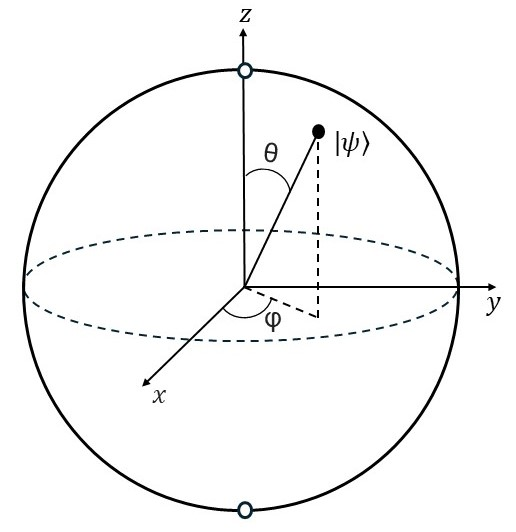
\includegraphics[width=0.4\textwidth]{images/bloch_sphere.jpg}
  \caption{Bloch sphere representation of a qubit}
  \label{fig:bloch_sphere}
\end{figure}

The distance between two quantum states $\ket{\psi}$ and $\ket{\psi'}$ is their Euclidean distance in the Bloch sphere \cite{wallman2016noise,nielsen2010quantum}. 

There are infinite points in the Bloch sphere, which might suggest the possibility of encoding an infinite amount of information in the infinite binary expansion of the angle $\theta$. However, when a qubit is measured, it collapses to one of the basis states, so only one bit of information can be extracted from a qubit. To accurately determine the amplitudes $\alpha$ and $\beta$, an infinite number of identical qubit copies would need to be measured. Nevertheless, it is still conceptually valid to think of these amplitudes as ``hidden information''. One could say that quantum computation is the art of manipulating this hidden information using phenomena such as interference and superposition to perform tasks that would be impossible or inefficient with classical computers.


% Nota sobre parte final do chuang: informação codificada num qubit e o que perdemos qd medimos um qubit
% Computação quantica é a arte de manipular a informação escondida nos estados quanticos (fenomenos como interferencia e superposição) para realizar tarefas que seriam impossiveis ou ineficientes com computadores clássicos.

\subsection{Multi-qubit States} \label{subsec:entanglement}

 The state space of a composite physical system is the tensor product of the state spaces of the component physical systems. As a result, an $n$-qubit state can be represented by a unit vector in $2^n$-dimensional Hilbert space, $\mathbb{C}^{2^{n}}$. The notations \gls{states-otimes}, \gls{states-no-otimes}, and \gls{states-2gether} are  used to denote the tensor product of two states $\ket{\psi}$ and $\ket{\phi}$. As for any complex vector, $\ket{\psi}^{\otimes n}$ denotes the n-fold tensor product of state $\ket{\psi}$ with itself. The computational basis states of an $n$-qubit system are of the form $\ket{x_{1}\ldots x_{n}}$ and so a quantum state of such a system is specified by $2^{n}$ amplitudes. For instance, a two-qubit state can be written as
\begin{equation*}
  \ket{\psi} = \alpha_{00}\ket{00} + \alpha_{01}\ket{01} + \alpha_{10}\ket{10} + \alpha_{11}\ket{11}.
\end{equation*}

It should be noted that unfortunately, no simple generalization of the Bloch sphere known for multiple qubits.

%falta n-fold
%ir ao tensor e acrecentar os operadores que mapeiam operadores

\subsubsection{Entanglement}
An interesting aspect of multi-qubit states is the phenomenon of \emph{entanglement}. This term means strong intrinsic correlations between two (or more) particles when the quantum state of each of them cannot be described independently of the state of the other, \text{i.e.} cannot be written as a product of states of the individual qubits. Measuring one qubit of the entangled pair affects the state of the other qubit. This must happen even if the particles are far apart.

In order to better understand this concept, consider the follow \emph{Bell state} or \emph{EPR pair}:
\begin{equation*}
  \ket{\Phi^{+}} = \frac{1}{\sqrt{2}}(\ket{00} + \ket{11}).
\end{equation*}

Upon measuring the first qubit, there are two possible outcomes: $0$ with probability $1/2$ and $1$ with probability $1/2$. If the first qubit is measured to be $0$, the second qubit will also be $0$ with probability 1. If the first qubit is measured to be $1$, the second qubit will also be $1$ with probability 1. Therefore, the measurement outcomes are correlated.

These correlations prompted Einstein, Podolsky, and Rosen to publish a paper \cite{einstein1935can} questioning the completeness of quantum mechanics in 1935. The EPR paradox presented a dilemma: the existence of entanglement (\text{i.e.}, correlations that persist regardless of distance) versus local realism and hidden variables. Einstein argued that if two objects, which have interacted in the past but are now separated, exhibit perfect correlation, they must possess a set of properties determined before their separation. These properties would persist in each object, dictating the outcomes of measurements on both sides. Einstein believed that the strong correlations predicted by quantum mechanics necessitate the existence of additional properties not accounted for by the quantum formalism that determine the measurement results. Therefore, he argued that quantum mechanics might require supplementation, as it may not represent a complete or ultimate description of reality.


In 1964, John Bell made a remarkable discovery: the measurement correlations in the Bell state are stronger than those that could ever occur between  classical systems \cite{bell1964einstein}. He explored the idea that each entangled particle might possess hidden properties — unaccounted for by quantum mechanics—that determine the measurement outcomes. Then, through mathematical reasoning, Bell demonstrated that the correlations predicted by any local hidden variable theory cannot exceed a specific level.  There is an upper limit of correlations fixed by what today is called the ``Bell inequalities". He found that quantum theory sometimes predicts correlations that exceed this limit. Consequently, an experiment could  settle the debate by testing whether or not correlations surpass the bounds he had found following Einstein's position.


In 1982, Alain Aspect conducted an experiment that confirmed the violation of the Bell inequalities \cite{aspect1982experimental}. In this experiment, polarizers were placed more than twelve meters apart. This meant that the correlation obtained could not be explained by the fact that the particles carry within them unmeasured properties. Moreover, it proved that the outcome of the measurement is not determined until the moment of measurement. There seemed to be an instantaneous exchange between two particles at the time of measurement when they were twelve meters apart.



Sixteen years later, Nicolas Gisin \cite{tittel1998experimental} and Anton Zeilinger \cite{pan1998experimental} conducted similar experiments, demonstrating that entanglement persists over distances of several kilometers. More recently,  \cite{yin2017satellite} extended these tests using entangled photon pairs sent from a satellite to verify Bell's inequalities over a distance of one thousand kilometers, further confirming that, regardless of the distance, entangled particles behave as an indivisible, inseparable whole. The connection between them is so profound that it appears to challenge the principles of relativity. This phenomenon is known as \emph{quantum nonlocality}.

\subsection{Unitary operators and Measurements}\label{subsec:unitary-operators&measurements}




\subsubsection{Pauli Matrices}
The Pauli matrices are a set of three $2 \times 2$ hermitian matrices that are defined as follows:
\begin{equation*}
  \sigma_{x} = \begin{pmatrix} 0 & 1\\ 1 & 0 \end{pmatrix}, \hspace{1cm} \sigma_{y} = \begin{pmatrix} 0 & -i\\ i & 0 \end{pmatrix}, \hspace{1cm} \sigma_{z} = \begin{pmatrix} 1 & 0\\ 0 & -1 \end{pmatrix}.
\end{equation*}

The eigenvectors and eigenvalues of the Pauli matrices are as follows:
\begin{align*}
 & \sigma_{x} \begin{pmatrix} 1 \\ 1 \end{pmatrix} = \begin{pmatrix} 1 \\ 1 \end{pmatrix}, \hspace{1.4cm} \sigma_{y} \begin{pmatrix} 1 \\ i \end{pmatrix} =  \begin{pmatrix} 1 \\ i \end{pmatrix}, \hspace{1.4cm} \sigma_{z} \begin{pmatrix} 1 \\ 0 \end{pmatrix} = \begin{pmatrix} 1 \\ 0 \end{pmatrix} \\
  & \sigma_{x} \begin{pmatrix} 1 \\ -1 \end{pmatrix} = -\begin{pmatrix} 1 \\ -1 \end{pmatrix}, \hspace{0.7cm} \sigma_{y} \begin{pmatrix} 1 \\ -i \end{pmatrix} = -\begin{pmatrix} 1 \\ -i \end{pmatrix}, \hspace{0.7cm} \sigma_{z} \begin{pmatrix} 0 \\ 1 \end{pmatrix} = -\begin{pmatrix} 0 \\ 1 \end{pmatrix}.
\end{align*}

The normalized eigenvectors of $\sigma_x$ are $\ket{+} = \frac{1}{\sqrt{2}}(\ket{0} + \ket{1})$ and $\ket{-} = \frac{1}{\sqrt{2}}(\ket{0} - \ket{1})$, and normalized eigenvectors of $\sigma_y$ are $\ket{+i} = \frac{1}{\sqrt{2}}(\ket{0} + i\ket{1})$ and $\ket{-i} = \frac{1}{\sqrt{2}}(\ket{0} - i\ket{1})$. The eigenvectors of $\sigma_z$ are $\ket{0}$ and $\ket{1}$. These eigenvectors correspond to the $\hat{x}, \hat{y}$ and $\hat{z}$ axes of the Bloch sphere in \autoref{fig:bloch_sphere}, respectively.

When matrices $\sigma_x, \sigma_y$ or  $\sigma_z$ are applied to a state on the Bloch sphere, they rotate the state by $\pi$ radians around the $\hat{x}, \hat{y}$ or $\hat{z}$ axis, respectively. For example, the action of $\sigma_x$ on the state $\ket{0}$ is to rotate it to $\ket{1}$, and vice versa. Note that for the eigenstates of these matrices with eigenvalue $-1$, this still applies if considering a global phase of $-1 = e^{i\pi}$, given that two quantum states $\ket{\psi}$ and $e^{i\phi}\ket{\psi}$ are indistinguishable by any quantum measurement.

Matrices $\sigma_x$ and $\sigma_z$ will also be referred to as \gls{x} and \gls{z}, respectively.

\subsubsection{Unitary operators}
Closed systems, \text{i.e.}, systems that do not interact with other systems evolve according to unitary operators. In quantum computation, these unitary operators are also known as \emph{gates}. For a  state $\ket{\psi}$, a unitary operator $U$ describes an evolution from $\ket{\psi}$ to $ U\ket{\psi}$.

Pauli matrices are examples of unitary operators. The $X$ and $Z$ gates are often referred to as the \emph{not} and \emph{phase flip} gates, respectively. Other important unitary operators include   \emph{Hadamard gate}, denoted \gls{h}, which maps $\ket{0}$ to $\ket{+}$ and $\ket{1}$ to  $\ket{-}$, and the \emph{phase-shift gate}, denoted \gls{p}, which leaves $\ket{0}$ unaltered applies a phase shift of $\theta$ to the state $\ket{1}$:
\begin{equation*}
 H = \frac{1}{\sqrt{2}}\begin{pmatrix} 1 & 1\\ 1 & -1 \end{pmatrix}, \hspace{1cm} P = \begin{pmatrix} 1 & 0\\ 0 & e^{i \theta} \end{pmatrix}.
\end{equation*}
 
When the Pauli matrices are exponentiated, they result in three valuable classes of unitary matrices, corresponding to the rotation operators around the $\hat{x}$, $\hat{y}$, and $\hat{z}$ axes, which are defined as follows:
\begin{equation*}
  R_{x}(\theta) = e^{-i\theta \sigma_{x}/2} = \text{cos} \left(\frac{\theta}{2} \right) I -i \text{sin} \left(\frac{\theta}{2} \right) \sigma_{x} = \begin{pmatrix} \cos(\frac{\theta}{2}) & -i\sin(\frac{\theta}{2})\\ -i\sin(\frac{\theta}{2}) & \cos(\frac{\theta}{2}) \end{pmatrix},
\end{equation*}
\begin{equation*}
  R_{y}(\theta) = e^{-i\theta \sigma_{y}/2} = \text{cos} \left(\frac{\theta}{2} \right) I -i \text{sin} \left(\frac{\theta}{2} \right) \sigma_{y} = \begin{pmatrix} \cos(\frac{\theta}{2}) & -\sin(\frac{\theta}{2})\\ \sin(\frac{\theta}{2}) & \cos(\frac{\theta}{2}) \end{pmatrix},
\end{equation*}
\begin{equation*}
  R_{z}(\theta) = e^{-i\theta \sigma_{z}/2} = \text{cos} \left(\frac{\theta}{2} \right) I -i \text{sin} \left(\frac{\theta}{2} \right) \sigma_{z} = \begin{pmatrix} e^{-i\theta/2} & 0\\ 0 & e^{i\theta/2} \end{pmatrix}.
\end{equation*}

\begin{theorem} \label{unitary} \cite{nielsen2010quantum}
  Suppose $U$ is a unitary operation on a single qubit. Then there exist real numbers $\alpha$, $\beta$, $\gamma$ and $\delta$ such that
  \begin{equation*}
    U = e^{i\alpha} R_{z}(\beta) R_{y}(\gamma) R_{z}(\delta).
  \end{equation*}
\end{theorem}

There are also multi-qubit gates, such as the \emph{controlled-not} gate, denoted \gls{cnot}, which leaves the states $\ket{00}$ and  $\ket{01}$ unchanged, and maps $\ket{10}$ and $\ket{11}$ to each other:
\begin{equation*}
  \textit{CNOT} = \begin{pmatrix} 1 & 0 & 0 & 0\\ 0 & 1 & 0 & 0\\ 0 & 0 & 0 & 1\\ 0 & 0 & 1 & 0 \end{pmatrix}.
\end{equation*}
In this case, as the state of the first qubit determines if the $X$ gate is applied to the second qubit, the first qubit is called the \emph{control qubit} and the second qubit the \emph{target qubit}. 

There is an ``extension" of the controlled-not gate, the controlled-$U$ gate, where $U$ is a unitary gate acting on a single qubit. This gate applies the gate $U$ to the target qubit if the control qubit is in state $\ket{1}$ and does nothing otherwise. It is defined as:
\begin{align*}
  &\textit{CU} (\ket{0} \otimes \ket{\psi}) = \ket{0} \otimes \ket{\psi}\\ 
  &\textit{CU} (\ket{1} \otimes \ket{\psi}) = \ket{1} \otimes U\ket{\psi}.
\end{align*}

It should be noted that no completely closed systems exist in the universe. Nevertheless, for many systems, the approximation of a closed system is valid.
% No fim nota sobre não haver sistemas completamente fechados no universo, mas que a aproximação de um sistema fechado é válida para muitos sistemas, p.82



\subsubsection{Measurements}

% decidir se e como por M0 e M1

There are times when it necessary to observe the system to extract information. This interection leaves the system no longer closed and, consequently, the evolution of the system is no longer unitary. 

The act of measuring a qubit is represented by a set of operators called \emph{measurement operators}, denoted $\{M_{m}\}$. These operators act on the state space  of the system being measured. The index $m$ refers possible measurement outcomes. These measurement operators must satisfy the completeness equation $\sum_{m} M_{m}^{\dagger}M_{m} = I$, which ensures that the probabilities of all possible outcomes sum to 1. If a measurement ${M_m}$ is performed on a state $\ket{\psi}$ the outcome $m$ is observed with probability $p_m = \bra{\psi}M_{m}^{\dagger}M_{m}\ket{\psi}$ for each $m$. Moreover, after a measurement yielding outcome $m$, the state collapses to $\frac{M_{m}\ket{\psi}}{\sqrt{p_{m}}}$. 

In the case of the computational basis, the measurement operators are the projectors onto the basis states $\ket{0}$ and $\ket{1}$ denoted by $M_{0} = \ket{0}\bra{0}$ and $M_{1} = \ket{1}\bra{1}$, respectively. Considering an arbitrary state $\ket{\psi} = \alpha \ket{0} + \beta \ket{1}$, the probabilities of measuring 0 and 1 are $p_0 = \bra{\psi} M_{0} M_{0}^{\dag}\ket{\psi}=\bra{\psi} M_{0} \ket{\psi} = |\alpha|^{2}$, and $p_1 = \bra{\psi} M_{1} M_{1}^{\dag}\ket{\psi} = \bra{\psi} M_{1} \ket{\psi} =  |\beta|^{2} $. Consequently the states after measurement are $\frac{M_{0}\ket{\psi}} {|\alpha|} = \frac{\alpha}{|\alpha|} \ket{0} = \ket{0}$ (with $p=p_0$) and $\frac{M_{1}\ket{\psi}} {|\beta|} = \frac{\beta}{|\beta|} \ket{1} = \ket{1}$ (with $p=p_1$).

From now on, unless stated otherwise, any reference to measurement should be understood as pertaining to the computational basis.

As previously mentioned, any states $\ket{\psi}$ and $e^{i\phi}\ket{\psi}$ are indistinguishable by any quantum measurement. Consider a measurement operator $M_m$, the probabilities of obtaining outcome $m$ are $\bra{\psi} M_{m}^{\dagger}M_{m}\ket{\psi}$ and $\bra{\psi} e^{-i \theta} M_{m}^{\dagger}M_{m}e^{i\theta}\ket{\psi}=\bra{\psi} M_{m}^{\dagger}M_{m}\ket{\psi}$. For this reason, it is said that these states are equal from an observational point of view.



%If a measurement ${M_m}$ is performed on a state $\rho$, the outcome $m$ is observed with probability $p_m = \text{Tr}(M_{m} \rho M^{\dag}_{m})$ for each $m$. Moreover, after a measurement yielding outcome $m$, the state collapses to $M_{m}\rho M^{\dag}_{m}/p_{m}$. 
% ver p.93

\subsection{Density operators}
Until now the state vector formalism was used. However there is an alternative formulation using density operators. The density operator is often known as the \emph{density matrix}, the two terms will be used interchangeably.

%\subsubsection{General properties}


A quantum state $\ket{\psi}$ is said to be a \emph{pure state} if it is completely known, \text{i.e.} if it can be written as a ket. In this case, the state can be written in the density operator formalism as $\rho = \ket{\psi}\bra{\psi}$. On the other hand, a state that is a probabilistic mixture of pure states is designated a \emph{mixed state}. A mixed state $\sum_i \alpha_i \ket{\psi_i}$ can be represented by a density operator $\rho= \sum_i |\alpha_i|^{2}\ket{\psi_i}\bra{\psi_i}$. Note that $|\alpha_i|^{2}$ is the probability of the system being in state $\ket{\psi_i}$. 

With respect to density operators, when applying a unitary operator $U$ to a state $\rho$, the resulting state is $U\rho U^{\dag}$. Regarding measurements, given a collection of measurement operators, $\{M_{m}\}$, the probability of obtaining outcome $m$ is $p(m)=\text{Tr}(M_{m}\rho M_{m}^{\dag})$, and after a measurement yielding outcome $m$, the state collapes to  $\frac{M_{m}^{\dag}\rho M_{m}}{\text{Tr}(M_{m}\rho M_{m}^{\dag})}$.

In \autoref{subsec:hilb2D} it was shown how to determine the cartesian coordenates of a pure state in the Bloch Sphere from the state vector. For an arbitrary $2 \times 2$ density matrix, the following holds
\begin{equation} \label{eq:bloch_vector_0}
  \rho = \frac{1}{2}(I + r_{x}\sigma_{x} + r_{y}\sigma_{y} + r_{z}\sigma_{z}),
\end{equation} 

where $\vec{r} = (r_x, r_y, r_z)$ is a real three-dimensional vector such that $\| \vec{r} \|_2 \leq 1$. This vector is known as the Bloch vector for the state $\rho$. Since $\rho$ is Hermitian. $r_x, r_y$ and $r_z$ are always real.  The inverse map of \autoref{eq:bloch_vector_0} is
\begin{equation}
  \label{eq:Bloch_vector}
  r_{\mu} = \text{Tr}(\rho \sigma_{\mu})
  \end{equation}

  Note that given that the trace is linear and matrix multiplication distributes over matrix addition, the cartesian coordinates of an operator consisting of the sum or subtraction of density operators can also be determined by \autoref{eq:Bloch_vector}.

\subsubsection{Reduced density operator}

Density operators are particularly well-suited for describing individual subsystems of a composite quantum system. This type of description is provided by the \emph{reduced density operator}

Given physical systems $A$ and $B$ whose composite system is given by the density operator $\rho_{AB}$, the reduced density operator for subsystem $A$ is $$\rho_{A} = \text{Tr}_{B}(\rho_{AB}),$$ where $ \text{Tr}_{B}$ is the partial trace over the Hilbert space of subsystem $B$, defined as 
\begin{align*}
  \text{Tr}_{B}(\ket{a_1}\bra{a_2} \otimes \ket{b_1}\bra{b_2}) & =\ket{a_1}\bra{a_2}\text{Tr}(\ket{b_1}\bra{b_2}) \\
  & = \ket{a_1}\bra{a_2}  \sum_{\mu} \bra{\mu} \ket{b_1}\bra{b_2} \ket{\mu} \\
  & =  \ket{a_1} \bra{a_2} \sum_{\mu} \braket{\mu} {b_1}\braket{b_2} {\mu} \\
  & = \ket{a_1} \bra{a_2} \sum_{\mu} \braket{b_2}{\mu} \braket{\mu}{b_1} \\
  &= \ket{a_1}\bra{a_2}  \braket{b_2}{b_1}
\end{align*}
 where $\ket{a_1}$ and $\ket{a_2}$ are any two vectors in the state space of $A$,  $\ket{b_1}$ and $\ket{b_2}$ are any two vectors in the state space of $B$, and $\{\ket{\mu}\}$, span the state space of $B$.  Therefore, by linearly, the partial trace of $\rho_{AB} = \sum_{ijkl} p_{ijkl} \ket{a_i} \bra{a_j}  \otimes \ket{b_k} \bra{b_l}$ is
\begin{align*}
  \text{Tr}_{B}(\rho_{AB}) &= \sum_{ijkl} p_{ijkl} \text{Tr}_{B}\left(\ket{a_i}\bra{a_j} \otimes \ket{b_k} \bra{b_l}\right) \\
  & = \sum_{ijkl} p_{ijkl} \ket{a_i}\bra{a_j}  \sum_{\mu} \braket{b_l}{\mu} \braket{\mu}{b_k}= \sum_{ijkl} p_{ijkl} \ket{a_i}\bra{a_j}   \braket{b_l}{b_k} 
  %& = \sum_{ijkk} p_{ijkk} \ket{a_i}\bra{a_j} = \sum_{ij} \overline{p_{ij}} \ket{a_i}\bra{a_j}
\end{align*} 
%Where, in the third line, it is assumed that $\{b_k\}$ forms an orthonormal basis, and $\overline{p_{ij}}= \sum_{k}p_{ijkk}$. The expression obtained.
To demonstrate that this operator is a density operator, it must be shown that it possesses unit trace and is positive semidefinite. Given that the trace of $\rho_{AB}$ corresponds to the sum of the diagonal elements of the density matrix, $\sum_i{ik} p_{iikk}$, and that that is also the case for the reduced density operator $\rho_{A}$, the sum of the diagonal elements is preserved by the partial trace. Thus, $\rho_{a}$ has trace equal to 1.  Moreover, considering that %$\rho_{AB}$ is a density operator, one has that
\begin{align*}
  &\langle \ket{\psi}, \rho_{AB} \ket{\psi} \rangle = \bra{\psi} \rho_{AB} \ket{\psi} = \bra{\psi} \sum_{ijkl} p_{ijkl} \ket{a_i} \bra{a_j}  \otimes \ket{b_k} \bra{b_l} \ket{\psi} \\ 
  = &\sum_{ijkl} p_{ijkl} \bra{\psi} \ket{a_i} \bra{a_j}  \otimes \ket{b_k} \bra{b_l} \ket{\psi} \\
  = & \sum_{ijkl} p_{ijkl} \sum_m (\alpha_{m}^{*} \bra{a_m} \otimes \bra{b_m}) \ket{a_i} \bra{a_j} \otimes \ket{b_k} \bra{b_l}  \sum_m (\alpha_{m}  \ket{a_m} \otimes \ket{b_m} )\\
  = & \sum_{ijklm} p_{ijkl} |\alpha_m|^{2} \braket{a_m}{a_i} \braket{a_j}{a_m} \braket{b_m}{b_k} \braket{b_l}{b_m} \\
  = & \sum_{ijkl}  p_{ijkl}  \braket{a_j}{a_i} \braket{b_l}{b_k} \\
\end{align*}
and that,
\begin{align*}
  &\langle \ket{\psi}, \rho_{A} \ket{\psi} \rangle = \bra{\psi} \rho_{A} \ket{\psi}
  = \bra{\psi} \sum_{ijkl} p_{ijkl} \ket{a_i}\bra{a_j} \braket{b_l}{b_k} \ket{\psi} \\
  = & \sum_{ijkl} p_{ijkl}  \braket{b_l}{b_k}  \bra{\psi} \ket{a_i}\bra{a_j}\ket{\psi} = \\
  = & \sum_{ijklm} p_{ijkl} \braket{b_l}{b_k} \sum_m (\alpha_{m}^{*} \bra{a_m}) \ket{a_i}\bra{a_j} \sum_m (\alpha_{m}  \ket{a_m} ) \\
  = & \sum_{ijklm} p_{ijkl} \braket{b_l}{b_k} |\alpha_m|^{2} \braket{a_m}{a_i} \braket{a_j}{a_m} = \sum_{ijkl} p_{ijkl} \braket{b_l}{b_k} \braket{a_j}{a_i} \\
  = & \sum_{ijkl} p_{ijkl}  \braket{a_j}{a_i} \braket{b_l}{b_k}
\end{align*}
where, $\{\ket{a_m}\}$ span the space of $A$ and $\{\ket{b_m}\}$ span the space of $B$, it is possible to conclude that $\langle \ket{\psi}, \rho_{AB} \ket{\psi} \rangle = \langle \ket{\psi}, \rho_{A} \ket{\psi} \rangle$. Thus, since $\langle \ket{\psi}, \rho_{AB} \ket{\psi} \rangle \geq 0$, the same applies to $\langle \ket{\psi}, \rho_{A} \ket{\psi} \rangle$. Therefore, $\rho_{A}$ is a positive semidefinite, and, consequently, a density operator.

% Note that TrB can also de expressec as I_A \otimes Tr (\rho_AB), where I_A is the identity operator in the Hilbert space of A.

In certain situations it is more advantageous to consider the reduced density operator for subsystem $A$ defined as:
\begin{equation*}
  \rho_{A} = \text{Tr}_{B}(\rho_{AB}) = \sum_{\mu} \bra{\mu} \rho_{AB} \ket{\mu},
\end{equation*}
where $\{\ket{\mu}\}$, span the state space of $B$ and act only in the state space of $B$. 

Similarly, the reduced density operator for subsystem $B$ is $\rho_{B} = \text{Tr}_{A}(\rho_{AB})$.


 %\begin{align*}
 %\text{Tr}_{B}(\ket{a}\bra{b} \otimes \ket{c}\bra{d}) & =\ket{i}\bra{j} \text{Tr}(\ket{k}\bra{l}) \\
 %&= \ket{a}\bra{b} \sum_{\mu} \bra{\mu} \ket{c}\bra{d}  \ket{\mu} \\
 %& = \sum_{\mu} \bra{\mu} \ket{a} \bra{b} \otimes \ket{c} \bra{d} \ket{\mu} 
%\end{align*}
%where $\ket{a}$ and $\ket{b}$ are any two vectors in the state space of $A$,  $\ket{c}$ and $\ket{d}$ are any two vectors in the state space of $B$, and $\{\ket{\mu}\}$, span the state space of $B$, act only in the state space of $B$. Therefore, by linearly, the partial trace of $\rho_{AB} = \sum_{ij} p_{ij} \ket{a_i} \bra{b_i}  \otimes \ket{c_j} \bra{d_j}  $ is




%An $n$-qubit mixed state can be represented by a density operator $ \mathbb{C}^{2^{n}} \xrightarrow{} \mathbb{C}^{2^{n}}$, whose matrix representation is $\rho = \Sigma_{i} \hspace{2pt} p_{i} \vert \phi_{i} \rangle \langle \phi_{i} \vert$. A density operator encodes uncertainty about the current state of the quantum system at hand. For example, a mixed state with half probability of $\vert 0 \rangle$ and $\vert 1 \rangle$ can be represented by $\frac{\vert 0 \rangle \langle 0 \vert + \vert 1 \rangle \langle 1 \vert}{2}=I/2$, where $I$ is the identity matrix.  One usually denotes density matrices by the greek letters $\rho$, $\sigma$, and so forth. The set of density operators is denoted by $\mathcal{D}_{n} \subseteq \mathbb{C}^{ 2^{n \times n}}$.

% tudo sobre matrizes de densidade incuindo a definição de matriz de densidade reduzida e traço parcial

% bloch vector for mixed states

\subsection{Quantum Channels} \label{subsec:quantum_channels}

% Fazer secção chamada quantum chanels e falar de super operadores e cptp maps, normas, kraus operators

Thus far, only two types of quantum operations have been discussed: unitary operators, which describe the evolution of a closed quantum system, and measurements, which describe the act of observing a quantum system. Now, a new type of quantum operation that accounts for the more realistic notion of interaction between a quantum system and an environment will be introduced. Nonetheless, it is necessary to first introduce a few key concepts.



%the evolution of a quantum system has been described by unitary operators. However, in practice, quantum systems are not isolated, and they interact with their environment. This interaction is described by a \emph{quantum channel}, which is a completely positive trace-preserving (CPTP) linear map. A quantum channel is a generalization of a unitary operator that allows for the description of the evolution of a quantum system under the influence of an environment.

\begin{definition}
  A \emph{super-operator} $Q$ is a linear map between the space of operators on a Hilbert space $E: \mathbb{C}^{n\times n} \rightarrow  \mathbb{C}^{m\times m}$. 
\end{definition}

\begin{definition} \label{def:positive_superoperator}
  A super-operator $Q$ is called \emph{positive} if it sends positive matrices to positive matrices, \textit{i.e.} $A \geq 0 \Rightarrow{} Q A \geq 0$.
\end{definition}

\begin{definition} \label{def:completely_positive_superoperator}
  A super-operator is said to be \emph{completely positive} if for all $k$, $Q \otimes I_{\mathbb{C}^{k \times k}}: \mathbb{C}^{n \times n} \otimes \mathbb{C}^{k \times k} \rightarrow \mathbb{C}^{m \times m} \otimes \mathbb{C}^{k \times k}  $ is positive.
\end{definition}

\begin{definition}
  A super-operator $Q$ is called \emph{trace-preserving} if $\text{Tr} \hspace{2pt} (Q A)= \text{Tr} (A)$.
\end{definition}

Since density matrices are positive, any physically allowed transformation must be represented by a positive operator. Moreover, this is not sufficient on its own: since one can always extend the space $\mathbb{C}^{n \times n}$ to  $\mathbb{C}^{n \times n} \otimes \mathbb{C}^{k \times k} $ by adjoining a new quantum system, any physically allowed transformation must be completely positive. Finally, since the trace of a density matrix is always $1$, any physically allowed transformation must be trace-preserving. A \acrfull{cptp} operator is traditionally called a \emph{quantum channel}.

\subsubsection{Kraus operator sum representation}
Assume that there is a quantum system $S$ of interest which is a subsystem of a larger system which also includes an environment $E$. These systems have a joint unitary evolution described by a unitary operator $U$ acting on the composite system, $U = \rho_{SE} \mapsto U \rho_{SE} U^{\dag}$. 

Given that density matrices are positve operators, by (\autoref{def:positive}), the density operator of the environment $\rho_E$ initially can be written as 
\begin{equation*}
  \rho_E = \sum_{i} p_{i} \ket{i} \bra{i}
\end{equation*}
where $\ket{i}$ form an orthonormal basis for the state space of $E$ and $p_{i}$ are positive. 

The state of the subsystem $S$ after the unitary evolution corresponds to the partial trace of the joint state over the environment,
\begin{align*}
  \rho_{S} = & \text{Tr}_{E}(U \rho_{SE} U^{\dag}) \\
 = & \sum_{\mu} \bra{\mu} U \rho_{SE} U^{\dag} \ket{\mu}
\end{align*}
where $\{\ket{\mu}\}$ span the state space of $E$.

 
Considering that initially both systems are completely decoupled, the initial state of the system can be written as $ \rho_{SE} = \rho_{S} \otimes \rho_{E}$. Thus,
\begin{align*} 
  \rho_{S} = & \sum_{\mu} \bra{\mu} U \rho_{S} \otimes \sum_{i} p_{i} \ket{i} \bra{i} U^{\dag} \ket{\mu} \\
  = & \sum_{\mu i}  \sqrt{p_{i}} \bra{\mu} U \ket{i} \rho_{S} \sqrt{p_{i}} \bra{i} U^{\dag} \ket{\mu}  \\ 
  = & \sum_{\mu i} \text{K}_{\mu i} \rho_{S} \text{K}_{\mu i}^{\dag}
\end{align*}
where the set of operators $\{\text{K}_{\mu i}\}$ is designated \emph{Kraus operators} and $\text{K}_{\mu i} = \sqrt{p_{i}} \bra{\mu} U \ket{i}$. Note that $\{\ket{\mu}\}$ and $\{\ket{i}\}$, act only in the state space of $E$. The equation $ \rho_{S} = \sum_{\mu i} \text{K}_{\mu i} \rho_{S} \text{K}_{\mu i}^{\dag} $ is called an \emph{\acrfull{osr}}.

\acrshort{osr} can be thought of as a quantum channel that maps $\rho_{S}$ to $\sum_{\mu i} \text{K}_{\mu i} \rho_{S} \text{K}_{\mu i}^{\dag}$, given this map is \acrshort{cptp} \cite{lidar2019lecture}. 

\subsubsection{Non-selective measurements}

In the previously presented formalism to represent all the possible outcomes of a measurement, described by a set of operators $\{M_{m}\}$, on a state $\rho$, it would be necessary to write that state $\rho$ collapse to state $\rho_m=\frac{M_{m}^{\dag}\rho M_{m}}{\text{Tr}(M_{m}\rho M_{m}^{\dag})}$ with probability $p(m)=\text{Tr}(M_{m}\rho M_{m}^{\dag})$, for each possible outcome $m$. However, this is not appropriate for calculations. Consequently, to better represent the effect of a measurement on a quantum system \emph{non-selective measurements} are used. In this case, the possible outcomes are not explicitly stated, and the state after the measurement is as follows:
\begin{equation*}
  \rho = \sum_{m} p_m \rho_m = \sum_{m} M_m \rho M^{\dag}_m
\end{equation*}
This last equality corresponds to an Kraus operator sum representation, where the set of Kraus operators is $\{M_{m}\}$.

% in the previouly presented formalism to express the resukt of a mesurment in a state we would have to say it is state x with probability px and y with probability py. However, this is not appropriate to perform calculations with. 


%For every super-operator $ E: \mathcal{D}(n) \xrightarrow{} \mathcal{D}(m)$, there exists a set of Kraus operators $\{\epsilon_{k}\}_{k}$ such that $ E(\rho)= \Sigma_{k} \hspace{2pt} \epsilon_{k}\hspace{2pt} \rho \hspace{2pt} \epsilon_{k}^{\dag}$  for any input $\rho \in  \mathcal{D}(n) $. Note that the set of Kraus operators is finite if the Hilbert space is finite-dimensional. The Kraus form of $E$ is written as $E = \Sigma_{k} \hspace{2pt} \epsilon_{k} \circ  \epsilon_{k}^{\dag}$.



\subsubsection{Norms on quantum channels}
\begin{definition}
  The norm of a super-operator $Q: \mathbb{C}^{n\times n} \xrightarrow{} \mathbb{C}^{m\times m }$ is defined:
  \begin{equation} 
    \lVert Q \rVert_{1} =  \max\{\lVert Q \hspace{1pt} A \rVert_{1} \hspace{2pt}  \vert \hspace{2pt}  \lVert A \rVert_{1}=1\}, 
  \end{equation}
\end{definition}
where $A \in \mathbb{C}^{n \times n }$

\begin{theorem} \label{thm:Russo–Dye} \cite[Theorem 3.39]{watrous2018theory}
  Let $Q: \mathbb{C}^{n \times n} \rightarrow \mathbb{C}^{m \times m}$ be a positive super-operator. It holds that 
  \begin{equation}
    \lVert Q \rVert_{1} = \max \{ \text{Tr}\left(Q(uu^{*}) \right) \vert \hspace{2pt}  \lVert u \rVert_{1}=1 \}.
  \end{equation}
\end{theorem}


\begin{proposition} \cite[Proposition 3.41]{watrous2018theory}
The following facts hold for the trace norm:
\begin{enumerate}
  \item The trace norm is submultiplicative with respect to composition of super-operators , \textit{i.e.}, for all super-operators  $Q: \mathbb{C}^{n \times n} \rightarrow \mathbb{C}^{m \times m}$ and $S: \mathbb{C}^{m \times m} \rightarrow \mathbb{C}^{o \times o}$
  \begin{equation}
    \lVert S  Q \rVert_{1} \leq \lVert S \rVert_{1} \lVert Q \rVert_{1}.
  \end{equation}
  \item Let $U_0,$ $V_0 \in \mathbb{C}^{n\times n}$ and $U_1,$ $V_1 \in \mathbb{C}^{m\times m}$ be unitary operators, let $Q,$ $S: \mathbb{C}^{n \times n} \rightarrow \mathbb{C}^{m \times m}$ be super-operators, where $S$ is defined as:
  \begin{equation}
    S(X) = U_1 Q(U_0 A V_0) V_1
  \end{equation}
  for all $A \in \mathbb{C}^{n\times n}$. It holds that $\lVert Q \rVert_{1} = \lVert S \rVert_{1} $.
\end{enumerate}
\end{proposition}

Unfortunately, this norm is not stable under tensoring , given that the inequation $ \lVert Q \otimes \text{I} \rVert_{1} \leq \lVert Q \rVert_{1}$ does not hold \cite{watrous2018theory}. As a result, the diamond norm, which is based on the trace norm, is used instead in the context of quantum channels. 

\begin{definition}
  Given a super-operator $Q: \mathbb{C}^{n\times n} \xrightarrow{} \mathbb{C}^{m\times m }$, the diamond norm, \gls{diamond-norm} , is defined as:
  \begin{equation}  \label{eq:diamond_distance}
    \lVert Q \rVert_{\diamondsuit} =  \lVert Q \otimes I_{\mathbb{C}^{n \times n}} \rVert_{1}
  \end{equation}
\end{definition}
%where $I_{\mathbb{C}^{n \times n}} $ is the identity super-operator over the space $\mathbb{C}^{n\times n}$.

%3.46
%For all super-operators $Q: \mathbb{C}^{n \times n}\rightarrow \mathbb{C}^{m \times m} $, it holds that 
%\begin{equation}
  %\lVert Q \rVert_{\diamondsuit} \geq \lVert Q \otimes I_{\mathbb{C}^{o\times o}} \rVert_{1},
%\end{equation}
%if $\text{dim}(\mathbb{C}^{o\times o}) \geq \text{dim}(\mathbb{C}^{n\times n})$.

For this norm it holds that for all super-operators $Q: \mathbb{C}^{n \times n}\rightarrow \mathbb{C}^{m \times m} $ and $S:\mathbb{C}^{m \times m} \rightarrow \mathbb{C}^{o \times o} $, if $Q$ is a quantum channel then $\lVert S  Q \rVert_{\diamondsuit} \leq \lVert S \rVert_{\diamondsuit}$ \cite[Proposition 3.44 and Proposition 3.48]{watrous2018theory}, and if $S$ is a quantum channel, then $\lVert S  Q \rVert_{\diamondsuit} \leq \lVert Q \rVert_{\diamondsuit}$. This is a desireble property, as is guarantees that quantum operations do not increase the distance between states, and as a
consequence, composition of programs is valid.
%Moreover, the following inequalties hold for a super-operator $Q$: $ \lVert Q \rVert_{\diamondsuit} \geq \lVert Q \otimes I \rVert_{\diamondsuit} $ and $\lVert Q \rVert_{\diamondsuit} \geq \lVert I \otimes Q  \rVert_{\diamondsuit} $
%3.44
\begin{proposition} \cite[Proposition 3.44]{watrous2018theory}
   For all quantum channels $Q:\mathbb{C}^{n \times n}\rightarrow \mathbb{C}^{m \times m}$, it holds that $\lVert Q \rVert_{\diamondsuit} = 1$.
\end{proposition}

\begin{theorem} \cite[Theorem 3.46 ]{watrous2018theory}
For all super-operators $Q:\mathbb{C}^{n \times n}\rightarrow \mathbb{C}^{m \times m}$ and complex spaces $\mathbb{C}^{o\times o}$  it holds that:
\begin{equation}
  \lVert Q \otimes I_{\mathbb{C}^{o\times o}} \rVert_{1} \leq  \lVert Q \rVert_{\diamondsuit}. 
\end{equation}
with equality holding under the assumption that $\text{dim}(\mathbb{C}^{o\times o}) \geq  \text{dim}(\mathbb{C}^{n \times n})$.
\end{theorem}

\begin{corollary} \label{cor:diamond_otimes_I} \cite[Corollary 3.47]{watrous2018theory}
   For all super-operators $Q:\mathbb{C}^{n \times n}\rightarrow \mathbb{C}^{m \times m}$ and complex spaces $\mathbb{C}^{o\times o}$  it holds that:
  \begin{equation}
    \lVert Q \rVert_{\diamondsuit} = \lVert Q \otimes I_{\mathbb{C}^{o\times o}} \rVert_{\diamondsuit} .
  \end{equation}
\end{corollary}

\begin{proposition} \cite[Proposition 3.48]{watrous2018theory}
  Moreover the following properties hold for the diamond norm:
  \begin{enumerate}
    \item The diamond norm is submultiplicative with respect to composition of , \textit{i.e.}, for all super-operators $Q: \mathbb{C}^{n \times n} \rightarrow \mathbb{C}^{m \times m}$ and $S: \mathbb{C}^{m \times m} \rightarrow \mathbb{C}^{o \times o}$, it holds that:
  \begin{equation}
    \lVert S  Q \rVert_{\diamondsuit} \leq \lVert S \rVert_{\diamondsuit} \lVert Q \rVert_{\diamondsuit}.
  \end{equation}
  \item For all super-operators $Q_0, S_0: \mathbb{C}^{n \times n} \rightarrow \mathbb{C}^{m \times m}$ and $Q_1, S_1: \mathbb{C}^{m \times m} \rightarrow \mathbb{C}^{o \times o}$, it holds that:
  \begin{equation}
  \lVert S_1 S_0 - Q_1 Q_0  \rVert_{\diamondsuit} \leq \lVert S_0 - Q_0 \rVert_{\diamondsuit} + \lVert S_1 - Q_1 \rVert_{\diamondsuit}.
  \end{equation}
\end{enumerate}
\end{proposition}

\begin{theorem} \cite[Theorem 3.49]{watrous2018theory}
  \item The diamond norm is multiplicative with respect to tensor products, \textit{i.e.}, for all super-operators $Q: \mathbb{C}^{n \times n} \rightarrow \mathbb{C}^{m \times m}$ and $S: \mathbb{C}^{o \times o} \rightarrow \mathbb{C}^{p \times p}$, it holds that:
  \begin{equation}
    \lVert Q \otimes S \rVert_{\diamondsuit} = \lVert Q \rVert_{\diamondsuit} \lVert S \rVert_{\diamondsuit}.
  \end{equation}
\end{theorem}


Consider an operator  $ \text{r} : (\mathbb{C}^{n} \xrightarrow[]{} \mathbb{C}^{m}) \xrightarrow[]{} (\mathbb{C}^{n\times n}\xrightarrow[]{} \mathbb{C}^{m\times m})$ that sends an operator $T$ to the mapping $A \mapsto TAT^{\dag}$. The exact calculation of distances induced by $\lVert \rVert_{\diamondsuit}$ tends to be quite complicated, but a useful property for calculating the distance between quantum channels in the image of $r$ is provided in \cite{watrous2018theory}.
Consider two operators $T, S : n \xrightarrow{} m$. There exists a unit vector $v \in \mathbb{C}^{n}$ such that, 
\begin{equation} \label{eq:norm_iso_r}
\begin{centering}
\lVert r(T) (vv^{\dag})-r(S) (vv^{\dag}) \rVert_{1} = \lVert r(T)-r(S) \rVert_{\diamondsuit}
 \end{centering}
\end{equation}

\subsection{Quantum circuits}
As quantum computation remains in its early stages of development, programming is primarily based on the use of \emph{quantum circuits}. A quantum circuit consists of wires and \emph{quantum gates}, which serve to transmit and manipulate quantum information. Each wire corresponds to a qubit, while the gates represent operations that can be applied to these qubits. 

In this subsection the notation for the quantum gates used in this work will be introduced.

Wires in parallel represent the tensor product of the respective qubits. For instance, $\psi_0 \otimes \psi_1$ corresponds to
\begin{figure} [H]
  \centering
  \begin{quantikz} [column sep=0.5cm, row sep=0.8cm] 
      \lstick{$\ket{\psi_0}$} & \qw & \qw & \qw \\
      \lstick{$\ket{\psi_1}$} & \qw & \qw & \qw 
 \end{quantikz}
\end{figure}

The single bit gates presented in \Cref{subsec:unitary-operators&measurements} are represented as a box with the symbom of the gate inside. For example, the Hadamard gate is represented as
\begin{figure} [H]
  \centering
  \begin{quantikz} [column sep=0.5cm, row sep=0.8cm] 
       & \gate{H} & \qw
 \end{quantikz}
\end{figure}

The controlled-not gate, which is a two-qubit gate, is represented as
\begin{figure} [H]
  \centering
  \begin{quantikz} [column sep=0.5cm, row sep=0.8cm] 
      & \ctrl{1} & \qw \\
       & \targ{} & \qw 
 \end{quantikz}
\end{figure}

Similarly, the controlled-$U$ gate, where $U$ is an unitary single-qubit gate, is represented as
\begin{figure} [H]
  \centering
  \begin{quantikz} [column sep=0.5cm, row sep=0.8cm] 
      & \ctrl{1} & \qw \\
       & \gate{U} & \qw 
 \end{quantikz}
\end{figure}

An arbitrary unitary operator acting on $n$ qubits is represented as a box acting on $n$ wires. For instance, the operator $U$ acting on two qubits is represented as
\begin{figure} [H]
  \centering
  \begin{quantikz} [column sep=0.5cm, row sep=0.8cm] 
      & \gate[wires=2]{U} & \qw \\
      & &\qw
 \end{quantikz}
\end{figure}

\acrshort{cptp} maps are depicted as boxes containing the corresponding map symbols. The relevant \acrshort{cptp} operators will be introduced in \autoref{subsec:noisy_teleportation}.

The measurement operation is representes by a ``meter'' symbol. Given that output of a measurement is a classical bit, the wire representing the output of a measurement is a classical wire, representes by a double line. 

\begin{figure} [H]
  \centering
  \begin{quantikz} [column sep=0.5cm, row sep=0.8cm] 
      & \meter{} & \setwiretype{c}  
 \end{quantikz}
\end{figure}



\subsection{No-cloning theorem}
The no-cloning theorem states that it is impossible to duplicate an unknown quantum bit \cite{wootters1982single}. In this subsection, an elementary proof of this theorem will be presented.

Suppose that there exists a unitary operator $U$ that recieves a qubit $\ket{\psi}$ and some standard pure state $\ket{s}$ as input and oututs the state $\ket{\psi} \otimes \ket{\psi}$. The action of $U$ can be written as
\begin{equation*}
  U \left(\ket{\psi} \otimes \ket{s} \right) = \ket{\psi} \otimes \ket{\psi}
\end{equation*}
Consider the aplication of $U$ to two pure states $\ket{\psi_0}$ and $\ket{\psi_1}$,
\begin{align*}
  U \left(\ket{\psi_0} \otimes \ket{s} \right) = \ket{\psi_0} \otimes \ket{\psi_0} \\
  U \left(\ket{\psi_1} \otimes \ket{s} \right) = \ket{\psi_1} \otimes \ket{\psi_1}.
\end{align*}

Given that unitary operators preserve inner products, the following equality should hold:
\begin{equation*}
  \braket{\psi_0}{\psi_1} = ( \braket{\psi_0}{\psi_1})^{2}
\end{equation*}

This equation is only satisfied if $\braket{\psi_0}{\psi_1} = 0$ or $\braket{\psi_0}{\psi_1} = 1$. The first case implies that $\ket{\psi_0}$ and $\ket{\psi_1}$ are orthogonal, and the second case implies that they are in the same state. Therefore, it is only possible to clone orthogonal states. These are the states perfectly distinguishable by measurement and thus are equivalent to copying classical information. For instance, it is impossible to the clone qubits $\psi_0 = \ket{0}$ and $\psi_1 = \ket{-}$, since they are not orthogonal.

It should be noted that this principle is upheld by the type system outlined in \autoref{fig:typing_rules_linear}, which does not allow the repeated use of a variable (seen as a quantum resource).




\section{Interpretation} \label{sec:Quantum Lambda Calculus:Interpretation}
The syntax of the metric lambda calculus was presented in \Cref{ch:metriclambda}. Now, it is necessary to define the \emph{model} of the ``reality'' of interest, \textit{i.e.}, what the terms of the calculus mean within the ``reality'' considered. In the case of quantum lambda calculus, the model is based on quantum channels. The interpretation introduced in this subsection is based on the work of \cite{dahlqvist2022syntactic} with the addition of the measurement operation.
% o outro modelo vai ser baseado em somas diretas de espaços vetoriais e quantum channels

%and $!_{V}: V \xrightarrow{} \mathbb{C}$ is the trace operation applied to a vector, defined as  $!_{V}= v \xrightarrow{} \text{Tr} \hspace{1pt}v$.

In order to define the interpretation of judgments $\Gamma \triangleright v: \mathbb{A}$, it is necessary to establish some notation first. Considering $v \in V$, $w \in W$, and $r \in R$  where $V, W, R$ represent vector spaces,  $\textsc{sw}_{V,W} : V\otimes W \xrightarrow{} W \otimes V$, denotes the swap operator, defined as $\textsc{sw}_{V,W}= v\otimes w \mapsto w \otimes v$;    $\lambda_{V} : \mathbb{C} \otimes V \xrightarrow{} V $ is the left unitor defined as $\lambda_{V}= 1 \otimes v \mapsto v $; $\rho_{V} : V  \otimes \mathbb{C} \xrightarrow{} V $ is the right unitor defined as $\rho_{V}= v \otimes 1 \mapsto v$; and $\alpha_{V,W,R} : V  \otimes (W \otimes R) \xrightarrow{} (V  \otimes W) \otimes R$ is the left associator, defined as $\alpha_{V,W,R}= v \otimes (w \otimes r) \mapsto (v \otimes w) \otimes r $. Moreover, for all operators $f: V \otimes W \xrightarrow{} R$, the operator $\overline{f} : V \xrightarrow{} (W \multimap R)$ denotes the corresponding curried version, defined as $\overline{f}(v) = w \mapsto  f(v,w)$. On the other hand, the application operator denoted $\text{app}: (V \multimap W) \otimes V \rightarrow W$, is defined as $f\hspace{1pt} v = w $, where $f: V \multimap W $.   The subscripts in these operators will be omitted unless ambiguity arises. 

For all ground types $X \in G$  the interpretation of $[\![X]\!]$  is postulated as a vector space $V$. Types are interpreted inductively using the unit $\mathbb{I}$, the tensor $\otimes$, and the linear map $\multimap$. Given a non-empty context $\Gamma=\Gamma',x: \mathbb{A}$, its interpretation is defined by $[\![\Gamma',x: \mathbb{A}]\!] = [\![\Gamma']\!] \otimes [\![\mathbb{A}]\!]$ if $\Gamma'$ is non-empty and $[\![\Gamma',x: \mathbb{A}]\!] = [\![\mathbb{A}]\!]$ otherwise. The empty context $-$ is interpreted as $[\![-]\!] = [\![ \mathbb{I}]\!] = \mathbb{C}$. Given $X_{1}, . . . ,X_{n} \in V$, the $n$-tensor $(\ldots (X_1 \otimes X_2) \otimes \ldots ) \otimes X_{n}$ is denoted as $X_1 \otimes \ldots \otimes X_{n}$, and similarly for operators. 


``Housekeeping" operators are employed to handle interactions between context interpretation and the vectorial model. Given $\Gamma_{1}, \ldots, \Gamma_{n}$, the operator that splits $[\![\Gamma_{1}, \ldots, \Gamma_{n}]\!]$ into $[\![\Gamma_{1}]\!] \otimes \ldots \otimes [\![\Gamma_{n}]\!]  $ is denoted by $\text{sp}_{\Gamma_1;\ldots;\Gamma_n}: [\![\Gamma_{1}, \ldots, \Gamma_{n}]\!] \xrightarrow{} [\![\Gamma_{1}]\!] \otimes \ldots \otimes [\![\Gamma_{n}]\!] $. For $n=1$, $\text{sp}_{\Gamma_1} = \text{id}$.
Let $\Gamma_1$ and $\Gamma_2$ be two contexts, $\text{sp}_{\Gamma_1, \Gamma_2} \rightarrow \Gamma_1\otimes \Gamma_2$ is defined as:
\begin{equation*}
  \text{sp}_{-; \Gamma_2} = \lambda^{-1} \hspace{1cm} \text{sp}_{\Gamma_1; -} = \rho^{-1} \hspace{1cm} \text{sp}_{\Gamma_1;x:\mathbb{A}} = I \hspace{1cm} \text{sp}_{\Gamma_1; \Delta, x: \mathbb{A}} = \alpha \cdot (\text{sp}_{\Gamma_1; \Delta} \otimes I)
\end{equation*}
For $n>2$, $\text{sp}_{\Gamma_1;\ldots;\Gamma_n}$ is is defined recursively based on the previous definition, using induction on $n$:
\begin{equation*}
  \text{sp}_{\Gamma_1;\ldots;\Gamma_n} = (\text{sp}_{\Gamma_1;\ldots;\Gamma_{n-1}} \otimes I )\cdot \text{sp}_{\Gamma_1, \ldots, \Gamma_{n-1} ;\Gamma_n}
\end{equation*}
On the other hand, $\text{jn}_{\Gamma_1;\ldots;\Gamma_n}$ denotes the inverse of $\text{sp}_{\Gamma_1;\ldots;\Gamma_n}$. Next, given $\Gamma, x : \mathbb{A}, y : \mathbb{B},\Delta$, the operator permuting $x$ and $y$ is denoted by $\text{exch}_{\Gamma, x : \mathbb{A}, y : \mathbb{B},\Delta}: [\![\Gamma,\underline{ x : \mathbb{A}, y : \mathbb{B}},\Delta]\!] \xrightarrow{} [\![\Gamma, y : \mathbb{B}, x : \mathbb{A}, \Delta]\!] $ and defined as:
\begin{equation*}
  \text{exch}_{\Gamma, \underline{ x : \mathbb{A}, y : \mathbb{B}},\Delta} = \text{jn}_{\Gamma; y:\mathbb{B}, x:\mathbb{A};\Delta} \cdot (I \otimes \text{sw} \otimes I ) \cdot \text{sp}_{\Gamma; x:\mathbb{A}, y:\mathbb{B};\Delta}
\end{equation*} 


The shuffling operator $\text{sh}_{E}: [\![E]\!] \xrightarrow{} [\![\Gamma_1, \ldots, \Gamma_n ]\!]$ is defined as a suitable composition of exchange operators.


For every operation symbol $f: \mathbb{A}_{1}, \ldots, \mathbb{A}_{n} \xrightarrow{} \mathbb{A}$ it is assumed the existence of an operator $[\![f]\!]: [\![\mathbb{A}_{1}]\!] \otimes \ldots \otimes [\![\mathbb{A}_{n}]\!] \xrightarrow{}  [\![\mathbb{A}]\!] $.
The interpretation of judgments is defined by induction over derivations according to the rules in \autoref{fig:denotational_sem} \cite{dahlqvist2022syntactic}.
\vspace{-7pt}
\begin{figure} [H]
\begin{equation*}
\begin{split}
\begin{aligned}
&
\begin{minipage}[t]{0.3\textwidth}
$\begin{array}{c}
      [\![\Gamma_{i} \triangleright v_{i}: \mathbb{A}_{i} ]\!]=m_{i}  \quad f: \mathbb{A}_{1}, \ldots, \mathbb{A}_{n} \xrightarrow{} \mathbb{A} \in \Sigma \quad E \in \text{Sf}(\Gamma_{1}; \ldots; \Gamma_{n})\\
    \hline
  [\![E \triangleright f( v_{1},\ldots,v_{n}): \mathbb{A} ]\!] = [\![ f]\!] \cdot (m_{1}\otimes \ldots \otimes m_{n}) \cdot \text{sp}_{\Gamma_1;\ldots;\Gamma_n}\cdot \text{sh}_{E}
\end{array}
$
\end{minipage}
\hspace{208pt}
\begin{minipage}[t]{0.3\textwidth}
$\begin{array}{c}
      \\
    \hline
  [\![ x:\mathbb{A} \triangleright x:\mathbb{A}]\!] = \text{I}_{[\![\mathbb{A} ]\!]}
\end{array}
$ \end{minipage} \\
&
\begin{minipage}[t]{0.3\textwidth}
$\begin{array}{c}
     \\  
    \hline
   [\![ - \triangleright *: \mathbb{I}]\!] = \text{I}_{[\![\mathbb{I} ]\!]}
\end{array}
$
\end{minipage}
\hspace{-34pt}
\begin{minipage}[t]{0.3\textwidth}
$\begin{array}{c}
      [\![\Gamma \triangleright v: \mathbb{A} \otimes \mathbb{B} ]\!]=m  \quad [\![\Delta,x: \mathbb{A}, y: \mathbb{B}  \triangleright w: \mathbb{D} ]\!] =n  \quad E \in \text{Sf}(\Gamma;\Delta)\\
    \hline
  [\![ E\triangleright \text{pm } v \text{ to } x \otimes y. w :\mathbb{D}]\!] = n \cdot \text{jn}_{\Delta;\mathbb{A};\mathbb{B}} \cdot \alpha \cdot \text{sw}\cdot (m \otimes \text{I}) \cdot \text{sp}_{\Gamma;\Delta} \cdot \text{sh}_{E}
\end{array}
$ \end{minipage} \\
&
\begin{minipage}[t]{0.3\textwidth}
$\begin{array}{c}  
     [\![ \Gamma \triangleright v: \mathbb{A} ]\!] =m \quad [\![\Delta \triangleright w: \mathbb{B} ]\!]=n \quad E \in \text{Sf}(\Gamma;\Delta) \\
    \hline
  [\![ E \triangleright v \otimes w: \mathbb{A} \otimes \mathbb{B} ]\!] = (m \otimes n) \cdot \text{sp}_{\Gamma;\Delta} \cdot \text{sh}_{E}
\end{array} 
$
\end{minipage}\\
&
 \begin{minipage}[t]{0.3\textwidth}
$\begin{array}{c} 
    [\![\Gamma \triangleright v: \mathbb{I} ]\!]=m  \quad [\![\Delta \triangleright w: \mathbb{A}]\!]=n \quad E \in \text{Sf}(\Gamma;\Delta)  \\
    \hline
  [\![E \triangleright v \text { to } *.w: \mathbb{A} ]\!]=n \cdot \lambda \cdot (m \otimes \text{I}) \cdot \text{sp}_{\Gamma;\Delta} \cdot \text{sh}_{E}
\end{array}
$ \end{minipage} 
\hspace{130 pt}
\begin{minipage}[t]{0.3\textwidth}
$\begin{array}{c} 
     [\![\Gamma,x:\mathbb{A} \triangleright v: \mathbb{B} ]\!] = m \\
    \hline
   [\![ \Gamma \triangleright \lambda x:\mathbb{A} . \hspace{2pt } v: \mathbb{A} \multimap \mathbb{B}]\!] = \overline{m \cdot \text{jn}_{\Gamma;\mathbb{A}}}
\end{array}
$
\end{minipage} \\
&
 \begin{minipage}[t]{0.3\textwidth}
$\begin{array}{c} 
     [\![\Gamma \triangleright v: \mathbb{A} \multimap \mathbb{B} ]\!] = m \quad [\![  \Delta \triangleright w: \mathbb{A} ]\!] =n \quad E \in S\hspace{-3pt}f(\Gamma;\Delta)  \\
    \hline
  [\![ E \triangleright v w: \mathbb{B} ]\!] = \text{app} \cdot (m \otimes n) \cdot \text{sp}_{\Gamma;\Delta} \cdot \text{sh}_{E}
\end{array}
$ \end{minipage}
\hspace{190 pt} %[\![ ]\!]
\begin{minipage}[t]{0.3\textwidth}
$\begin{array}{c}
     [\![\Gamma \triangleright v: \mathbb{A}]\!]  = f \\
    \hline
   [\![ \Gamma \triangleright \text{dis}(v):  \mathbb{I} ]\!] = \text{Tr} \cdot f
\end{array}
$
\end{minipage}
\end{aligned}
\end{split}
\end{equation*}
\caption{Judgment interpretation}
\label{fig:denotational_sem} 
\end{figure}

The following diagrams are useful to better understand the interpretation of judgements given in \autoref{fig:denotational_sem}.
\begin{align*}
  & \llbracket \text{ax} \rrbracket : & [\![E]\!] & \xrightarrow{\hspace{2pt}\text{sh}_{E}\hspace{2pt}}   [\![\Gamma_1,\ldots,\Gamma_n ]\!]   \xrightarrow{\hspace{1pt}\text{sp}_{\Gamma;\Delta}\hspace{1pt}}  \llbracket \Gamma_1 \rrbracket \otimes \ldots \otimes \llbracket \Gamma_n \rrbracket  \\
  & & & \xrightarrow{\hspace{2pt}m_1 \otimes \ldots \otimes m_n \hspace{2pt}} \llbracket \mathbb{A}_1 \rrbracket \otimes \ldots \otimes \llbracket \mathbb{A}_n \rrbracket \xrightarrow{\hspace{2pt}\llbracket f \rrbracket \hspace{2pt}} \llbracket \mathbb{A} \rrbracket \\
  & \llbracket \text{hyp} \rrbracket : & \llbracket \mathbb{A} \rrbracket & \xrightarrow{\hspace{2pt}I_{\llbracket \mathbb{A}\rrbracket}\hspace{2pt}} \llbracket \mathbb{A}\rrbracket \\
  & \llbracket \mathbb{I}_i \rrbracket :&  \llbracket \mathbb{I} \rrbracket & \xrightarrow{\hspace{2pt}I_{\llbracket \mathbb{I}\rrbracket}\hspace{2pt}}  \llbracket \mathbb{I} \rrbracket\\
  &\llbracket \otimes_e \rrbracket : & [\![E]\!] & \xrightarrow{\hspace{2pt}\text{sh}_{E}\hspace{2pt}}   [\![\Gamma,\Delta ]\!]   \xrightarrow{\hspace{1pt}\text{sp}_{\Gamma;\Delta}\hspace{1pt}}  [\![\Gamma ]\!] \otimes [\![\Delta ]\!] \xrightarrow{ m \hspace{1pt} \otimes \hspace{1pt} \text{I}} ([\![\mathbb{A} ]\!] \otimes [\![\mathbb{B} ]\!]) \otimes [\![\Delta ]\!]   \\
     & &  &\xrightarrow{\hspace{2pt}\text{sw}\hspace{2pt}}  [\![\Delta ]\!] \otimes ([\![\mathbb{A} ]\!] \otimes [\![\mathbb{B} ]\!]) \xrightarrow{\hspace{3pt}\alpha\hspace{3pt}}  ([\![\Delta ]\!] \otimes [\![\mathbb{A} ]\!]) \otimes [\![\mathbb{B} ]\!] \xrightarrow{\hspace{2pt}\text{jn}_{\Delta; \mathbb{A}; \mathbb{B} }\hspace{2pt}}  \llbracket \Delta, \mathbb{A},\mathbb{B}  \rrbracket  \\
     &&& \xrightarrow{\hspace{3pt}n\hspace{3pt}} \llbracket \mathbb{D} \rrbracket \\
     &\llbracket \otimes_i \rrbracket : & [\![E]\!] & \xrightarrow{\hspace{2pt}\text{sh}_{E}\hspace{2pt}}   [\![\Gamma,\Delta ]\!]   \xrightarrow{\hspace{1pt}\text{sp}_{\Gamma;\Delta}\hspace{1pt}}  [\![\Gamma ]\!] \otimes [\![\Delta ]\!]  \xrightarrow{\hspace{2pt} m \hspace{1pt} \otimes \hspace{1pt} n \hspace{2pt}} [\![\mathbb{A} ]\!] \otimes [\![\mathbb{B} ]\!] \\
     &\llbracket \mathbb{I}_e \rrbracket :  & [\![E]\!] & \xrightarrow{\hspace{2pt}\text{sh}_{E}\hspace{2pt}}   [\![\Gamma,\Delta ]\!]   \xrightarrow{\hspace{1pt}\text{sp}_{\Gamma;\Delta}\hspace{1pt}}  [\![\Gamma ]\!] \otimes [\![\Delta ]\!] \xrightarrow{ m \hspace{1pt} \otimes \hspace{1pt} \text{I}} [\![\mathbb{I} ]\!]\otimes [\![\Delta ]\!] \xrightarrow{\hspace{2pt} \lambda \hspace{3pt}} [\![\Delta ]\!]  \xrightarrow{\hspace{2pt} n \hspace{3pt}}  \llbracket \mathbb{A} \rrbracket    \\
      &\llbracket \multimap_i \rrbracket : & \llbracket \Gamma \rrbracket \otimes \llbracket \mathbb{A} \rrbracket & \xrightarrow{\hspace{2pt} \overline{m \cdot \text{jn}_{\Gamma;\mathbb{A}}}  \hspace{2pt}}  \llbracket \mathbb{A} \rrbracket \multimap \llbracket \mathbb{B} \rrbracket  \hspace{60pt} (\llbracket \Gamma \rrbracket \otimes \llbracket \mathbb{A} \rrbracket  \xrightarrow{\hspace{2pt} \text{jn}_{\Gamma; \mathbb{A}} \hspace{2pt}} \llbracket \Gamma, \mathbb{A} \rrbracket  \xrightarrow{\hspace{2pt} m \hspace{2pt}}  \llbracket \mathbb{B} \rrbracket )\\
      &\llbracket \multimap_e \rrbracket : & [\![E]\!] & \xrightarrow{\hspace{2pt}\text{sh}_{E}\hspace{2pt}}   [\![\Gamma,\Delta ]\!]   \xrightarrow{\hspace{1pt}\text{sp}_{\Gamma;\Delta}\hspace{1pt}}  [\![\Gamma ]\!] \otimes [\![\Delta ]\!]  \xrightarrow{\hspace{2pt} m \hspace{1pt} \otimes \hspace{1pt} n \hspace{2pt}} \llbracket \mathbb{A} \rrbracket \multimap \llbracket \mathbb{B} \rrbracket \otimes \llbracket \mathbb{A} \rrbracket  \xrightarrow{\hspace{2pt} \text{app} \hspace{2pt}} \llbracket \mathbb{B} \rrbracket \\
      &\llbracket \text{dis} \rrbracket : & [\![\Gamma]\!] & \xrightarrow{\hspace{2pt} f \hspace{2pt}} \llbracket \mathbb{A} \rrbracket \xrightarrow{\hspace{2pt} \text{Tr} \hspace{2pt}} \llbracket \mathbb{I} \rrbracket
      %& \llbracket \Gamma \rrbracket \otimes \llbracket \mathbb{A} \rrbracket  \xrightarrow{\hspace{2pt} \text{jn}_{\Gamma; \mathbb{A}} \hspace{2pt}} \llbracket \Gamma, \mathbb{A} \rrbracket  \xrightarrow{\hspace{2pt} m \hspace{2pt}}  \llbracket \mathbb{B} \rrbracket 
\end{align*} 


Regarding the interpretation of the exhange and substitution properties, for any judgements $\Gamma, x: \mathbb{A}, y: \mathbb{B}, \Delta \triangleright v : \mathbb{D}$, $\Gamma, x: \mathbb{A} \triangleright v: \mathbb{B}$, and $\Delta \triangleright w: \mathbb{A}$, the following equations hold:
\begin{equation}
\begin{split}
  \llbracket \Gamma, x: \mathbb{A}, y: \mathbb{B}, \Delta \triangleright v : \mathbb{D} \rrbracket & = \llbracket \Gamma,  y: \mathbb{B}, x: \mathbb{A}, \Delta \triangleright v : \mathbb{D} \rrbracket \cdot \text{exch}_{\Gamma, \underline{x: \mathbb{A}, y: \mathbb{B}}, \Delta}\\
  \llbracket \Gamma,\Delta \triangleright v[w/x]: \mathbb{B} \rrbracket & = \llbracket \Gamma, x: \mathbb{A} \triangleright v: \mathbb{B} \rrbracket \cdot \text{jn}_{\Gamma;\mathbb{A}} \cdot (\text{I} \otimes \llbracket \Delta \triangleright w: \mathbb{A} \rrbracket ) \cdot \text{sp}_{\Gamma; \Delta} 
\end{split}
\end{equation}

\subsubsection{Types and operations in quantum lambda calculus}

In the case of quantum lambda calculus, it is natural to consider a type $\textit{qbit}$ of quantum bits.  The interpretation of this type is defined as $[\![\textit{qbit}]\!]=\mathbb{C}^{2\times 2}$. 

The following operations are considered: the creation of a new qubit in the state $\ket{0}$, $\textit{new} \hspace{2pt} 0 :\mathbb{I} \multimap \textit{qbit}$, the creation of a new qubit in the state $\ket{1}$ ($\textit{new} \hspace{2pt} 1 :\mathbb{I} \multimap \textit{qbit}$), measuring a qubit, $\textit{meas}: \textit{qbit} \multimap \textit{qbit}$, applying a unitary operation to a qubit, $\textit{U}: \textit{qbit}^{\otimes n} \multimap \textit{qbit}^{\otimes n}$, and performing a \acrshort{cptp} operation on a qubit, $\textit{CPTP}: \textit{qbit}^{\otimes n} \multimap \textit{qbit}^{\otimes n}$. These operations are defined in \autoref{fig:interpret_ops_0}.

\begin{figure}[H]
  \begin{equation*}
  \begin{split}
  \begin{aligned}
  &
  \hspace{10pt}
  \begin{minipage}[t]{0.45\textwidth}
  $\begin{aligned}
    [\![\textit{new} \, 0 ]\!] : \hspace{2pt}& \mathbb{C} \multimap \llbracket \textit{bit} \rrbracket  \\
  & 1 \mapsto \big(\begin{smallmatrix}
    1 & 0\\
    0 & 0
  \end{smallmatrix}\big) 
  \end{aligned}$
  \end{minipage}
  \hspace{-70pt}
  \begin{minipage}[t]{0.45\textwidth}
  $\begin{aligned}
    [\![\textit{new} \, 1 ]\!] :\hspace{2pt}& \mathbb{C} \multimap \llbracket \textit{bit} \rrbracket  \\
    & 1 \mapsto \big(\begin{smallmatrix}
      0 & 0\\
      0 & 1
    \end{smallmatrix}\big)
  \end{aligned}$
  \end{minipage} 
  \hspace{-70pt}
  \begin{minipage}[t]{0.45\textwidth}
  $\begin{aligned}
    [\![\textit{meas}]\!]:\hspace{2pt} & \llbracket \textit{qbit} \rrbracket \multimap \llbracket \textit{bit} \rrbracket  \\
    &\rho \mapsto M_{0} \rho M_{0}^{\dag} +  M_{1} \rho M_{1}^{\dag} 
  \end{aligned}$
  \end{minipage} 
  \\
  &
  \hspace{10pt}
  \begin{minipage}[t]{0.45\textwidth}
    $\begin{aligned}
      [\![\textit{U} ]\!] : \hspace{2pt} & \llbracket \textit{qbit} \rrbracket^{\otimes n} \multimap \llbracket 
      \textit{qbit} \rrbracket^{\otimes n} \\
      & \rho \mapsto U \rho \hspace{2pt}  U^{\dag}
    \end{aligned}$
    \end{minipage} 
  \hspace{70pt}
  \begin{minipage}[t]{0.45\textwidth}
    $\begin{aligned}
      [\![\textit{CPTP} ]\!] : \hspace{2pt} & \llbracket \textit{qbit} \rrbracket^{\otimes n} \multimap \llbracket 
      \textit{qbit} \rrbracket^{\otimes n} \\
      & \rho \mapsto \textit{CPTP} (\rho)
    \end{aligned}$
    \end{minipage} \\
  \end{aligned}
  \end{split}
  \end{equation*}
  \caption{Judgment interpretation of the operations in quantum lambda calculus.}
  \label{fig:interpret_ops_0}
  \end{figure}


% Flar sobre o que é cptp e o que não é

The chosen model requires that all operators considered are \acrshort{cptp} maps. The identity $I$, the swap operator $\text{sw}$, the left and right unitors $\rho$ and $\lambda$, the left associator $\alpha$,the trace operation $!$, the split operator $\text{sp}$, the join operator $\text{jn}$, the exhange $\text{exch}$ and shuffle $\text{sh}$ are all  \acrshort{cptp} maps \cite{dahlqvist2022syntactic}. However, the operators curry $\overline{f}$ and application $\text{app}$ are not \acrshort{cptp} maps, which means that they are not allowed in this model. On the other hand the measurement operator $[\![\textit{meas}]\!]$ and the unitary operator $[\![\textit{U}]\!]$ are \acrshort{cptp} maps (\Cref{subsec:quantum_channels}, \cite[page 73]{watrous2018theory}). Finally, regarding the operators  $[\![\textit{new} \,0 ]\!]$ and $[\![\textit{new} \, 1 ] \!]$, it is straightforward to verify that the operators $ \llbracket \textit{new} \, 0 \rrbracket $ and $\llbracket\textit{new} \, 1 \rrbracket$ are trace-preserving. Given that matrices $\big(\begin{smallmatrix} 1 & 0\\ 0 & 0 \end{smallmatrix}\big)$ and $\big(\begin{smallmatrix} 0 & 0\\ 0 & 1 \end{smallmatrix}\big)$ correspond to the projectors $\ket{0}\bra{0}$ and $\ket{1}\bra{1}$, one has that 
\begin{align} \label{eq:prove_new_0}
  \hspace{-20pt} &  \bra{\psi} \ket{0}\bra{0} \otimes I^{\otimes n} \ket{\psi}  = \bra{\psi} \ket{0}\bra{0} \otimes \left(\frac{\ket{0}\bra{0} + \ket{1}\bra{1}}{2}\right)^{\otimes n} \ket{\psi} \\
  \hspace{-20pt} =  &  \sum_{i} |\alpha_i|^{2} \braket{\psi_{0i}}{0}\braket{0}{\psi_{0i}} \bra{\psi_{1i}} \left(\frac{\ket{0}\bra{0} + \ket{1}\bra{1}}{2}\right)\ket{\psi_{1i}} \ldots \bra{\psi_{ni}} \left(\frac{\ket{0}\bra{0} + \ket{1}\bra{1}}{2}\right)\ket{\psi_{ni}}   \\
  \hspace{-20pt} = & \sum_{i}  |\alpha_i|^{2} |\braket{0}{\psi_{0i}}|^{2} \left( \frac{ \left( |\braket{0}{\psi_{1i}}|^{2} +  |\braket{1}{\psi_{1i}}|^{2} \right) \ldots \left( |\braket{0}{\psi_{ni}}|^{2} +  |\braket{1}{\psi_{ni}}|^{2} \right) }{2}  \right)    \\
\end{align}
Given that the squared absolute value of a real number is always non-negative, the expression above is always non-negative. Therefore, the operator $[\![\textit{new} \,0 ]\!]$ is positive. The same reasoning can be applied to the operator $[\![\textit{new} \,1 ]\!]$. Therefore, attending to \autoref{def:completely_positive_superoperator} and \autoref{def:positive_superoperator}, it is possible to conclude that both operators $[\![\textit{new} \,0 ]\!]$ and $[\![\textit{new} \, 1 ] \!]$ are completely positive super-operators. As a result, both operators are \acrshort{cptp} maps.
%attending to \autoref{def:positive_superoperator} and \autoref{def:positive} given that both matrices $\big(\begin{smallmatrix} 1 & 0\\ 0 & 0 \end{smallmatrix}\big)$ and $\big(\begin{smallmatrix} 0 & 0\\ 0 & 1 \end{smallmatrix}\big)$ are hermitian and have eigenvalues $0$ and $1$, they are positive super-operators. 

  \subsection{Example: Deutsch's Algorithm}

  In 1985, David Deutsch presented an algorithm that determines whether a function $f$ is constant for a single-bit input (\textit{i.e.}, either equal to 1 for all $x$ or equal to 0 for all $x$) or balanced (\textit{i.e.}, equal to 1 for half of the values of $x$ and equal to 0 for the other half) \cite{deutsch1985quantum}. Classically, to determine which case holds requires running $f$ twice. Quantumly, it suffices to run f once. The Deutsch-Jozsa Algorithm is a simple example of a quantum algorithm that outperforms its classical counterpart. The algorithm is based on the concept of a quantum oracle, which is a black box that implements a unitary transformation $U_f$ such that $U_f \ket{x}\ket{y} = \ket{x}\ket{y \oplus f(x)}$, where $\oplus$ denotes addition modulo 2. The quantum circuit implementing Deutsch’s algorithm is presented in  \autoref{fig:Deutsch-Jozsa}.
  
  \begin{figure} [H]
    \centering
    \begin{quantikz} [column sep=0.2cm, row sep=0.5cm] 
      \lstick{$\ket{0}$} &  \qw & \gate{H} & \gate[wires=2]{U_f} & \gate{H} & \meter{} \\
      \lstick{$\ket{1}$} &  \qw & \gate{H} & \qw & \qw & \qw\\ 
    \end{quantikz}
    \caption{Quantum circuit implementing Deutsch’s algorithm}
    \label{fig:Deutsch-Jozsa}
  \end{figure}
  
  Using lambda calculus, the Deutsch-Jozsa Algorithm can be expressed as:
  \begin{align*}
  \text{Deutsch} =  - \triangleright & \hspace{3pt} \text{pm} \hspace{4pt}  U_{f}(H  \hspace{2pt}   ( \textit{new}   \hspace{2pt}  0 \hspace{1pt}(*)) \otimes H  \hspace{2pt}   ( \textit{new}   \hspace{2pt}  1 \hspace{1pt}(*))) \hspace{2pt}  \textit{to} \hspace{2pt} q_{1} \otimes q_{2} \hspace{1pt}. \\
  &\hspace{3pt} \textit{meas} (H( q_{1})) \otimes q_{2} : \textit{qbit} \otimes \textit{qbit}  \\ 
   \end{align*}

The proper interpretation of this term will be provided, but before that, an interpretation based on the quantum circuit in \autoref{fig:Deutsch-Jozsa} will be presented. 
%Here, the quantum state vector and density operator representations will be used interchangeably, according to what makes the calculations more simple.

Attending to the circuit in  \autoref{fig:Deutsch-Jozsa}, one has that
  \begin{equation} \label{eq:Deutsch-1H}
  \begin{split}
   & \ket{0} \otimes \ket{1} \\
   \xmapsto{ H \otimes H} \quad & \frac{1}{\sqrt{2}}(\ket{0} + \ket{1}) \otimes \ket{-} \\
  \end{split}
  \end{equation}
  
  With respecto to  quantum oracle $U_f$, it is possible to show that:
  \begin{equation}
  \begin{split}
    &\ket{x} \otimes \ket{-} =   \ket{x} \otimes \frac{1}{\sqrt{2}}(\ket{0} - \ket{1}) = \frac{1}{\sqrt{2}}(\ket{x} \otimes \ket{0} - \ket{x} \otimes \ket{1})) \\
    \xmapsto{ \hspace{2pt} U_{f} \hspace{2pt}} \hspace{4pt} &  \frac{1}{\sqrt{2}}(\ket{x} \otimes \ket{0 \oplus f(x)} - \ket{x} \otimes \ket{1 \oplus f(x)}) &\hspace{50pt} \{\text{Defn. of } U_f\} \\
    = \hspace{4pt}  & \frac{1}{\sqrt{2}}(\ket{x} \ket{f(x)} - \ket{x} \ket{\neg f(x)}) & \{0\oplus x=x, 1\oplus x = \neg x\} \\
    = \hspace{4pt}  & \frac{1}{\sqrt{2}}(\ket{x} \otimes (\ket{f(x)}-\ket{\neg f(x)}))
   \end{split}
  \end{equation}
  
  Proceding by case distinction:
  \begin{equation}
    \frac{1}{\sqrt{2}}(\ket{x} \otimes (\ket{f(x)}-\ket{\neg f(x)}) = 
    \begin{cases}
      \ket{x} \otimes \frac{1}{\sqrt{2}}(\ket{0}-\ket{1}) &\text{ if } f(x)=0    \\
      \ket{x} \otimes \frac{1}{\sqrt{2}}(\ket{1}-\ket{0}) &\text{ if }   f(x)= 1 
    \end{cases}
  \end{equation}
  
 It follows that:
  \begin{equation}
   \ket{x} \otimes  \frac{1}{\sqrt{2}}(\ket{f(x)}-\ket{\neg f(x)}) = (-1)^{f(x)} \ket{x} \otimes \frac{1}{\sqrt{2}}(\ket{0}-\ket{1}) = (-1)^{f(x)} \ket{x} \otimes \ket{-}
  \end{equation}
  
  Returning to the interpretation of the Deutsch Algorithm, one has that:
  \begin{align}
    \quad & \frac{1}{\sqrt{2}}(\ket{0} + \ket{1}) \otimes \ket{-}\\
    \xmapsto{ \hspace{5 pt} U_{f} \hspace{5pt}} \quad & \frac{1}{\sqrt{2}}( U_{f} \ket{0} \otimes \ket{-} + U_{f} \ket{1} \otimes \ket{-})) \\
    = \quad & \frac{1}{\sqrt{2}}( (-1)^{f(0)} \ket{0} \otimes \ket{-} + (-1)^{f(1)} \ket{1} \otimes \ket{-}) \label{eq:Deutsch-Uf} \\
    = \quad &
    \begin{cases}
      (\pm 1) \ket{+} \otimes \ket{-} &\text{ if }   f(0)= f(1) \\
      (\pm 1) \ket{-} \otimes \ket{-} &\text{ if }   f(0) \neq f(1)
    \end{cases} \label{eq:Deutsch-Uf_2} \\
    \xmapsto{ \hspace{2pt} H \otimes I \hspace{2pt}} \quad & 
    \begin{cases}
      (\pm 1) \ket{0} \otimes \ket{-} &\text{ if }   f(0)= f(1) \\
      (\pm 1) \ket{1} \otimes \ket{-} &\text{ if }   f(0) \neq f(1)\\
    \end{cases} \label{eq:Deutsch-H_final}
  \end{align} 
  Ignoring the global phase, the final state of the system is:
  \begin{equation} \label{eq:Deutsch-meas}
    \begin{split}
  \xmapsto{ \hspace{2pt} \textit{meas} \otimes I \hspace{2pt}} \quad &
  \begin{cases}
     \ket{0}  \otimes \ket{-}  &\text{ if }   f(0)= f(1) \\
    \ket{1}  \otimes \ket{-} &\text{ if }   f(0) \neq f(1) 
  \end{cases} \\
  \end {split}
\end{equation}

 %Switching to the density operator formalism,
  %\begin{equation}
    %\begin{split}
      %&\begin{cases}
        %\ket{0} \bra{0} \otimes \ket{-}  &\text{ if }   f(0)= f(1) \\
       %\ket{1}  \bra{1} \otimes \ket{-} &\text{ if }   f(0) \neq f(1) 
     %\end{cases} \\
  %\xmapsto{ \hspace{2pt} \textit{meas} \otimes I \hspace{2pt}} \quad &
  %\begin{cases}
     %\ket{0} \bra{0} \otimes \ket{-}  &\text{ if }   f(0)= f(1) \\
    %\ket{1}  \bra{1} \otimes \ket{-} &\text{ if }   f(0) \neq f(1) 
  %\end{cases} \\
  %\end {split}
%\end{equation} 

Now, regarding the interpretation of the lambda term \text{Deutch}, 
\begin{align*}
  \hspace{-25pt} &  \llbracket  \text{Deutch}\rrbracket \\
  \hspace{-25pt} = \hspace{2pt} & \llbracket - \triangleright  \hspace{3pt} \text{pm} \hspace{4pt}  U_{f}(H  \hspace{2pt}   ( \textit{new}   \hspace{2pt}  0 \hspace{1pt}(*)) \otimes H  \hspace{2pt}   ( \textit{new}   \hspace{2pt}  1 \hspace{1pt}(*))) \hspace{2pt}  \textit{to} \hspace{2pt} q_{1} \otimes q_{2} \hspace{1pt}.   \\
  \hspace{-25pt}& \hspace{1pt}\textit{meas} (H( q_{1})) \otimes q_{2} : \textit{qbit} \otimes \textit{qbit}   \rrbracket \\
  \hspace{-25pt} =  \hspace{2pt}  & \llbracket q_1:\textit{qbit} \otimes q_2:\textit{qbit}  \triangleright \textit{meas} (H( q_{1})) \otimes q_{2} : \textit{qbit} \otimes \textit{qbit} \rrbracket \cdot \text{jn}_{-;\textit{qbit}; \textit{qbit}}   &  \{\llbracket  \otimes_ e \rrbracket\}     \\
  \hspace{-25pt}&   \cdot \alpha \cdot \text{sw}  \cdot ( \llbracket - \triangleright U_{f}(H  \hspace{2pt}  ( \textit{new}   \hspace{2pt}  0 \hspace{1pt}(*)) \otimes H  \hspace{2pt}   ( \textit{new}   \hspace{2pt}  1 \hspace{1pt}(*))): \textit{qbit} \otimes \textit{qbit}  \rrbracket \\
  \hspace{-25pt}& \otimes I_{\mathbb{C}})   \cdot \text{sp}_{-;-}  \cdot  \text{sh}_{-;-} \\ 
  \hspace{-25pt} =  \hspace{2pt}  & (\llbracket q_1:\textit{qbit}\triangleright \text{meas}(H(q_1)): \textit{qbit} \rrbracket \otimes \llbracket q_2:\textit{qbit} \triangleright q_2:\textit{qbit} \rrbracket)  &  \{\llbracket  \otimes_i \rrbracket,  \\
  \hspace{-25pt}& \cdot \text{sp}_{\textit{qbit};\textit{qbit}} \cdot \text{sh}_{\textit{qbit};\textit{qbit}} \cdot \text{jn}_{-;\textit{qbit}; \textit{qbit}} \cdot \alpha  \cdot \text{sw}  \cdot ( \llbracket - \triangleright U_{f}(H  \hspace{2pt}  ( \textit{new}   \hspace{2pt}  0 \hspace{1pt}(*)) & \text{Def. sp and sh} \}  \\
  \hspace{-25pt}&  \otimes H  \hspace{2pt}   ( \textit{new}   \hspace{2pt}  1 \hspace{1pt}(*))) : \textit{qbit} \otimes \textit{qbit}  \rrbracket  \otimes I_{\mathbb{C}})  \cdot  I_{ \mathbb{C}} \otimes I_{\mathbb{C}} \cdot I_{\mathbb{C}} \otimes I_{\mathbb{C}}  \\
  \hspace{-25pt} =  \hspace{2pt} &  (\llbracket \text{meas} \rrbracket \cdot \llbracket H \rrbracket  \cdot \llbracket q_1:\textit{qbit} \triangleright q_1:\textit{qbit} \rrbracket \cdot \text{sp}_{\textit{qbit}} \cdot \text{sh}_{\textit{qbit}} \hspace{2pt}  \otimes I_{\llbracket \textit{qbit} \rrbracket})    &  \{\llbracket  \text{ax} \rrbracket, \llbracket  \text{hyp} \rrbracket \}  \\ 
  \hspace{-25pt} & \cdot \text{sp}_{\textit{qbit};\textit{qbit}} \cdot \text{sh}_{\textit{qbit};\textit{qbit}} \cdot \text{jn}_{-;\textit{qbit}; \textit{qbit}} \cdot \alpha \cdot \text{sw}\cdot (\llbracket U_f \rrbracket \cdot (\llbracket H \rrbracket   \otimes \llbracket H \rrbracket  \\
  \hspace{-25pt} &\cdot \llbracket  \textit{new}   \hspace{2pt}  0  \rrbracket \cdot  \llbracket - \triangleright *: \mathbb{I} \rrbracket \cdot \llbracket  \textit{new}   \hspace{2pt}  1  \rrbracket \cdot  \llbracket - \triangleright *: \mathbb{I} \rrbracket) \cdot \text{sp}_{-;-} \cdot  \text{sh}_{-} \otimes I_{\mathbb{C}})  \\
  \hspace{-25pt} =  \hspace{2pt} &   (\llbracket \text{meas} \rrbracket \cdot \llbracket H \rrbracket \cdot I_{\llbracket \textit{qbit} \rrbracket} \cdot I_{\llbracket \textit{qbit} \rrbracket}  \otimes I_{\llbracket \textit{qbit} \rrbracket} ) \cdot \text{sp}_{\textit{qbit};\textit{qbit}} \cdot \text{sh}_{\textit{qbit};\textit{qbit}}    &  \{\llbracket  \text{hyp} \rrbracket, \llbracket \mathbb{I}_i \rrbracket, \\
  \hspace{-25pt} & \cdot \text{jn}_{-;\textit{qbit}; \textit{qbit}} \cdot \alpha  \cdot \text{sw}\cdot ((\llbracket U_f \rrbracket \cdot (\llbracket H \rrbracket \cdot \llbracket  \textit{new}   \hspace{2pt}  0  \rrbracket \cdot I_{\mathbb{C}}  \otimes \llbracket H \rrbracket \cdot \llbracket  \textit{new}   \hspace{2pt}  1  \rrbracket & \text{Def. sp and sh} \}     \\
  &\cdot I_{\mathbb{C}}) \cdot  I_{\mathbb{C}} \otimes I_{\mathbb{C}} \cdot  I_{\mathbb{C}} \otimes I_{\mathbb{C}}) \otimes I_{\mathbb{C}})\\
  %\hspace{-25pt} =  \hspace{2pt} &   (\llbracket \text{meas} \rrbracket \cdot \llbracket H \rrbracket   \otimes I_{\llbracket \textit{qbit} \rrbracket} ) \cdot \text{sp}_{\textit{qbit};\textit{qbit}} \cdot \text{sh}_{\textit{qbit};\textit{qbit}} \cdot \text{jn}_{-;\textit{qbit}; \textit{qbit}} \cdot \alpha \cdot \text{sw}   &  \{\text{\autoref{fig:interpret_ops_0}} \} \\
  %& \cdot (\llbracket U_f \rrbracket \cdot (\llbracket H \rrbracket \cdot \ket{0}\bra{0} \otimes \llbracket H \rrbracket \cdot \ket{1}\bra{1} ) \otimes I_{\mathbb{C}})  \\
   \hspace{-25pt} =  \hspace{2pt} &  (\llbracket \text{meas} \rrbracket \cdot \llbracket H \rrbracket   \otimes I_{\llbracket \textit{qbit} \rrbracket} ) \cdot \text{sp}_{\textit{qbit};\textit{qbit}} \cdot \text{sh}_{\textit{qbit};\textit{qbit}} \cdot \text{jn}_{-;\textit{qbit}; \textit{qbit}} \cdot \alpha \cdot \text{sw}  &  \{\text{\autoref{fig:interpret_ops_0}} \}\\
   \hspace{-25pt} & \cdot (U_f \hspace{1pt} (H \ket{0}\bra{0} H^{\dag} \otimes H \ket{1}\bra{1} H^{\dag}) \hspace{1pt} U_f^{\dag} \otimes  I_{\mathbb{C}})  \\
   \hspace{-25pt} =  \hspace{2pt} &  (\llbracket \text{meas} \rrbracket \cdot \llbracket H \rrbracket   \otimes I_{\llbracket \textit{qbit} \rrbracket} ) \cdot \text{sp}_{\textit{qbit};\textit{qbit}} \cdot \text{sh}_{\textit{qbit};\textit{qbit}} \cdot \text{jn}_{-;\textit{qbit}; \textit{qbit}} \cdot \alpha \cdot \text{sw} &   \{\text{\autoref{eq:Deutsch-1H}}, \\
   \hspace{-25pt}& \cdot  \bigg( \left(\frac{1}{\sqrt{2}}( (-1)^{f(0)} \ket{0} \bra{0} \otimes \ket{-} \bra{-} + (-1)^{f(1)} \ket{1} \bra{1} \otimes \ket{-}\bra{-}) \right) & \text{\autoref{eq:Deutsch-Uf}}\}  \\
   & \otimes  I_{\mathbb{C}} \bigg) \\
   =  \hspace{2pt} &  (\llbracket \text{meas} \rrbracket \cdot \llbracket H \rrbracket   \otimes I_{\llbracket \textit{qbit} \rrbracket} ) \cdot \text{sp}_{\textit{qbit};\textit{qbit}} \cdot \text{sh}_{\textit{qbit};\textit{qbit}} \cdot \lambda \otimes I_{\mathbb{C}} \cdot \alpha  & \{ \text{Def. jn} \}\\
   & \cdot \bigg( I_{\mathbb{C}} \otimes  \bigg(\frac{1}{\sqrt{2}}( (-1)^{f(0)} \ket{0} \bra{0} \otimes \ket{-} \bra{-} + (-1)^{f(1)} \ket{1} \bra{1}  \\
   & \otimes \ket{-}\bra{-}) \bigg) \bigg) \\  
   =  \hspace{2pt} &  (\llbracket \text{meas} \rrbracket \cdot \llbracket H \rrbracket   \otimes I_{\llbracket \textit{qbit} \rrbracket} ) \cdot \bigg(\frac{1}{\sqrt{2}}( (-1)^{f(0)} \ket{0} \bra{0} \otimes \ket{-} \bra{-} &  \{\text{Def. sp and sh} \} \\
   & + (-1)^{f(1)} \ket{1} \bra{1} \otimes \ket{-}\bra{-}) \bigg) \bigg) \\
   %=  \hspace{2pt} & (M_0 \otimes I_{\llbracket \textit{qbit} \rrbracket})  \bigg(\frac{1}{\sqrt{2}}( (-1)^{f(0)} H\ket{0} H^{\dag}  \bra{0} \otimes  \ket{-} \bra{-} \\
   %& + (-1)^{f(1)} H \ket{1} \bra{1}  H^{\dag}\otimes \ket{-}\bra{-}) \bigg) (M_0^{\dag} \otimes I_{\llbracket \textit{qbit} \rrbracket})  \\
   %& + (M_1 \otimes I_{\llbracket \textit{qbit} \rrbracket})  \bigg(\frac{1}{\sqrt{2}}( (-1)^{f(0)} \ket{0} \bra{0} \otimes H \ket{-} \bra{-} H^{\dag} \\
   %& + (-1)^{f(1)} \ket{1} \bra{1} \otimes H \ket{-}\bra{-} H^{\dag}) \bigg) (M_1^{\dag} \otimes I_{\llbracket \textit{qbit} \rrbracket})  \\
   \hspace{2pt} = & \begin{cases}
    (M_0 \otimes I_{\llbracket \textit{qbit} \rrbracket}) \cdot (H\ket{+} \bra{+}H^\dag \otimes \ket{-}\bra{-})   &\text{ if }   f(0)= f(1) \\
    \cdot \hspace{2pt} (M_0^\dag \otimes I_{\llbracket \textit{qbit} \rrbracket}) + (M_1 \otimes I_{\llbracket \textit{qbit} \rrbracket})     \\
    \cdot \hspace{2pt} (H\ket{+} \bra{+}H^\dag \otimes \ket{-}\bra{-}) (M_1^\dag \otimes I_{\llbracket \textit{qbit} \rrbracket})\\
    (M_0 \otimes I_{\llbracket \textit{qbit} \rrbracket}) \cdot (H\ket{-} \bra{-}H^\dag \otimes \ket{-}\bra{-}) &\text{ if }   f(0) \neq f(1)\\
    \cdot \hspace{2pt} (M_0^\dag \otimes I_{\llbracket \textit{qbit} \rrbracket}) + (M_1 \otimes I_{\llbracket \textit{qbit} \rrbracket})  \\
     \cdot \hspace{2pt} (H\ket{-} \bra{-}H^\dag \otimes \ket{-}\bra{-}) (M_1^\dag \otimes I_{\llbracket \textit{qbit} \rrbracket})\\
   \end{cases} &   \begin{aligned}
    &\{\text{\autoref{eq:Deutsch-Uf_2}}, \\
    & \text{\autoref{fig:interpret_ops_0}}  \}
\end{aligned} \\
\hspace{2pt} = & 
\begin{cases}
  \ket{0} \bra{0}  \otimes \ket{-} \bra{-}  &\text{ if }   f(0)= f(1) \\
 \ket{1} \bra{1}  \otimes \ket{-} \bra{-} &\text{ if }   f(0) \neq f(1) 
\end{cases} 
&\begin{aligned}
  &\{\text{\autoref{eq:Deutsch-H_final}}, \\
  & \text{\autoref{eq:Deutsch-meas}}  \}
\end{aligned} \\
\end{align*}


\subsubsection{Deutsch's Algorithm with Measurement Errors}
  
  A measurement error is characterized by reading a "1" as a "0" or vice versa.  Measurement errors do not impact all states uniformly \cite{tannu2019mitigating}. Consequently, there is a discrepancy in how frequently the state "1" is incorrectly read as "0" compared to how often the state "0" is measured as "1" or vice versa.

  Given probabilities $p_1$ and $p_2$ of measuring a "0" as a "1" and a "1" as a "0", respectively, a measurement featuring this type of error, denoted $\text{meas}^{\epsilon}$, is defined as follows:
  \begin{equation}
    \begin{split}
      \text{meas}^{\epsilon}: &\llbracket \textit{qbit} \rrbracket \rightarrow \llbracket \textit{qbit} \rrbracket \\
    & \rho \mapsto (1-p_1)M_0 \rho M_0^{\dag} + (1-p_2) M_1 \rho M_1^{\dag} + p_1  M_1X\rho  X^{\dag}  M_1^{\dag} + p_2 M_0 X\rho X^{\dag} M_0^{\dag}
    \end{split}
  \end{equation}

Considering an arbitrary state $ \rho=|\alpha|^{2} |0\rangle \langle 0 | + \alpha \beta^{*} |0\rangle \langle 1 | + \alpha^{*} \beta |1\rangle \langle 0 | + |\beta|^{2} |1\rangle \langle 1 |$, the resulting state after measurement is:
\begin{equation}
  \begin{split}
    \text{meas}^{\epsilon} (\rho) & =  (1-p_1) |\alpha|^{2} |0\rangle \langle 0 | + (1-p_2)  |\beta|^{2} |1\rangle \langle 1 | + p_1 |\alpha|^{2} |1\rangle \langle 1 | + p_2 |\beta|^{2}  |0\rangle \langle 0 | \\
  & = ((1-p_1)|\alpha|^{2} + p_2 |\beta|^{2}) |0\rangle \langle 0 | + ((1-p_2) |\beta|^{2} + p_1 |\alpha|^{2}) |1\rangle \langle 1 | 
\end{split}
\end{equation}

Given that 
\begin{equation}
  \begin{split}
    \text{Tr} (\text{meas}^{\epsilon} (\rho))= &\text{Tr}(((1-p_1)|\alpha|^{2} + p_2 |\beta|^{2}) |0\rangle \langle 0 | + ((1-p_2) |\beta|^{2} + p_1 |\alpha|^{2}) |1\rangle \langle 1 |) \\
  =& (1-p_1)|\alpha|^{2} + p_2 |\beta|^{2} + (1-p_2) |\beta|^{2} + p_1 |\alpha|^{2} =  |\alpha|^{2} + |\beta|^{2} = \text{Tr}(\rho)
\end{split}
\end{equation}
this operator is trace-preserving. Attending to \autoref{eq:prove_new_0} and to the fact that the sum of positive semidefinite matrices is semidefinite (\autoref{def:positive}), it is straightforward to prove that the operator $\text{meas}^{\epsilon}$ is completely positive. As a result, $\text{meas}^{\epsilon}$ is a quantum channel and, consequently, a valid operation in the model considered.
  
  

%For example, considering $p_1=0.1$ and $p_2=0.3$ the resulting state after measurement is:
  %\begin{equation}
  %\begin{split}
    %\quad &
    %\begin{cases}
     %(0.9\ket{-} \bra{-},0.1\ket{-} \bra{-})  &\text{ if }   f(0)= f(1) \\
     %(0.3\ket{-} \bra{-}, 0.7\ket{-} \bra{-}) &\text{ if }   f(0) \neq f(1) 
    %\end{cases} \\
  %\end {split}
  %\end{equation}
  
  %As a result, the discrepancy between the ideal and actual measurement results corresponds to:
  %\begin{equation}
    %\begin{split}
      %\quad &
      %\begin{cases}
        %\lVert(\ket{-} \bra{-},0) - (0.9\ket{-} \bra{-},0.1\ket{-} \bra{-})   \rVert_{\diamondsuit} &\text{ if }   f(0)= f(1) \\
        %\lVert (0,\ket{-} \bra{-}) - (0.3\ket{-} \bra{-}, 0.7\ket{-} \bra{-}) \rVert_{\diamondsuit} &\text{ if }   f(0) \neq f(1) 
      %\end{cases} \\
      %= \quad &
      %\begin{cases}
        %\lVert(0.1\ket{-} \bra{-},-0.1\ket{-} \bra{-})   \rVert_{\diamondsuit} &\text{ if }   f(0)= f(1) \\
        %\lVert (-0.3\ket{-} \bra{-}, 0.3\ket{-} \bra{-}) \rVert_{\diamondsuit} &\text{ if }   f(0) \neq f(1)
      %\end{cases} \\
      %= \quad &
      %\begin{cases}
        %\lVert 0.1\ket{-} \bra{-}\rVert_{\diamondsuit} + \lVert - 0.1 \ket{-} \bra{-}\rVert_{\diamondsuit} &\text{ if }   f(0)= f(1) \\
        %\lVert -0.3\ket{-} \bra{-}\rVert_{\diamondsuit} + \lVert - 0.3 \ket{-} \bra{-}\rVert_{\diamondsuit} &\text{ if }   f(0) \neq f(1)
      %\end{cases} \\
    %\end {split}
    %\end{equation}
  
    %Employing \autoref{eq:Bloch_vector}, it is easily concluded that the Bloch vector of the state $\ket{-} \bra{-}$ is $(-1,0,0)$. Consequently,  the discrepancy between the ideal and actual measurement results is:
    %\begin{equation}
      %\begin{split}
        %& 
        %\begin{cases}
          %\lVert (-0.1,0,0) \rVert_{2} + \lVert (0.1,0,0) \ket{-} \bra{-}\rVert_{2} &\text{ if }   f(0)= f(1) \\
         % \lVert(0.3,0,0)\ket{-} \bra{-}\rVert_{2} + \lVert (-0.3,0,0) \ket{-} \bra{-}\rVert_{2} &\text{ if }   f(0) \neq f(1)
        %\end{cases} \\
        %= \quad &
        %\begin{cases}
          %\sqrt{(-0.1)^{2} + 0^{2} + 0^{2}} + \sqrt{(0.1)^{2} + 0^{2} + 0^{2}} &\text{ if }   f(0)= f(1) \\
          %\sqrt{(0.3)^{2} + 0^{2} + 0^{2}} + \sqrt{(-0.3)^{2} + 0^{2} + 0^{2}} &\text{ if }   f(0) \neq f(1)
        %\end{cases} \\
       % = \quad &
        %\begin{cases}
          %2 \sqrt{0.01} &\text{ if }   f(0)= f(1) \\
          %2 \sqrt{0.09}  &\text{ if }   f(0) \neq f(1)
        %\end{cases} \\
      %\end{split}
  %\end{equation}

  For example, considering $p_1=0.1$ and $p_2=0.3$ the resulting state after measurement is:
  \begin{equation}
  \begin{split}
    \rho'=\quad &
    \begin{cases}
     0.9 \ket{0} \bra{0}\ket{-} \bra{-} + 0.1 \ket{1} \bra{1} \ket{-} \bra{-}  &\text{ if }   f(0)= f(1) \\
     0.3 \ket{0} \bra{0} \ket{-} \bra{-} + 0.7 \ket{1} \bra{1} \ket{-} \bra{-} &\text{ if }   f(0) \neq f(1) 
    \end{cases} \\
  \end {split}
  \end{equation}
  
  As a result, the discrepancy between the ideal and actual measurement results,$\llbracket \rho - \rho' \rrbracket_{\diamondsuit} $, corresponds to:
  \begin{align}
    \quad & \llbracket \rho - \rho' \rrbracket_{\diamondsuit}  \\
      =\quad &
      \begin{cases}
        \lVert  (\ket{0} \bra{0}\ket{-} \bra{-} )- (0.9 \ket{0} \bra{0}\ket{-} \bra{-} + 0.1 \ket{1} \bra{1} \ket{-} \bra{-})  \rVert_{\diamondsuit} &\text{ if }   f(0)= f(1) \notag\\
        \lVert (\ket{1} \bra{1}  \ket{-} \bra{-}) - ( 0.3 \ket{0} \bra{0} \ket{-} \bra{-} + 0.7 \ket{1} \bra{1} \ket{-} \bra{-}) \rVert_{\diamondsuit} &\text{ if }   f(0) \neq f(1) 
      \end{cases} \notag\\
      = \quad &
      \begin{cases}
        \lVert 0.1 \ket{0} \bra{0}\ket{-} \bra{-} - 0.1\ket{1} \bra{1} \ket{-} \bra{-}   \rVert_{\diamondsuit} &\text{ if }   f(0)= f(1) \notag \\
        \lVert -0.3 \ket{0} \bra{0}\ket{-} \bra{-} + 0.3 \ket{1} \bra{1}\ket{-} \bra{-}   \rVert_{\diamondsuit} &\text{ if }   f(0) \neq f(1)
      \end{cases} \\
      = \quad &
      \begin{cases}
        \lVert 0.1 \hspace{1pt} (\ket{0} \bra{0} - \ket{1} \bra{1}) \ket{-} \bra{-}  \rVert_{\diamondsuit} &\text{ if }   f(0)= f(1) \notag \\
        \lVert  0.3  \hspace{1pt} (\ket{1} \bra{1} - \ket{0} \bra{0}) \ket{-} \bra{-}\rVert_{\diamondsuit} &\text{ if }   f(0) \neq f(1)
      \end{cases} \notag 
\end{align}
Attending to \autoref{def:norm} and the multiplicativity of the diamond norm with
respect to tensor products, it follows that:
\begin{align}
  \llbracket \rho - \rho' \rrbracket_{\diamondsuit} & = \hspace{2pt}
  \begin{cases}
    0.1  \lVert  \ket{0} \bra{0} - \ket{1} \bra{1}  \rVert_{\diamondsuit} \hspace{1pt}  \lVert  \ket{-} \bra{-}  \rVert_{\diamondsuit} &\text{ if }   f(0)= f(1) \notag \\
    0.3 \lVert  (\ket{1} \bra{1} - \ket{0} \bra{0}) \rVert_{\diamondsuit} \hspace{1pt}  \lVert \ket{-} \bra{-}\rVert_{\diamondsuit} &\text{ if }   f(0) \neq f(1)
  \end{cases} \notag  \\
\end{align}

      Employing \autoref{eq:Bloch_vector}, it is easily concluded that the Bloch vectors of the states $\ket{0} \bra{0}$, $\ket{1} \bra{1}$, and $\ket{-} \bra{-}$ are $(-1,0,0)$, $(0,0,1)$, and $(0,0,-1)$, respectively. Consequently, and considering \autoref{def:norm}  the discrepancy between the ideal and actual measurement results is:
    \begin{equation}
      \begin{split}
        \llbracket \rho - \rho' \rrbracket_{\diamondsuit} & = \hspace{2pt}
        \begin{cases}
          0.1 \lVert (0,0,1) \rVert_{2}  \hspace{1pt} \lVert (1,0,0)\rVert_{2}  &\text{ if }   f(0)= f(1) \\
          0.3\lVert(0,0,-2)\rVert_{2} \hspace{1pt}  \lVert (1,0,0)\rVert_{2} &\text{ if }   f(0) \neq f(1)
        \end{cases} \\
        = \hspace{2pt} &
        \begin{cases}
          0.2 \sqrt{1^{2} + 0^{2} + 0^{2}} \cdot \sqrt{1^{2} + 0^{2} + 0^{2}} &\text{ if }   f(0)= f(1) \\
          0.6\sqrt{(-1)^{2} + 0^{2} + 0^{2}} + \sqrt{1^{2} + 0^{2} + 0^{2}} &\text{ if }   f(0) \neq f(1)
        \end{cases} \\
        = \hspace{2pt} &
        \begin{cases}
         0.2 &\text{ if }   f(0)= f(1) \\
          0.6  &\text{ if }   f(0) \neq f(1)
        \end{cases} \\
      \end{split}
  \end{equation}
  
 % Via the metric deductive system in \autoref{fig:metric deductive system}, it is easily verified that if the distance between \textit{meas} and $\textit{meas}^{\epsilon}$ is $\epsilon$:s

For an arbitray distance $\epsilon$, between the ideal post-measurement state $\rho$ he erroneous post-measurement stat $\rho'$,  using the metric deductive system in \autoref{fig:metric deductive system} one can write:
  \begin{align*}
     \hspace{3pt} - \triangleright & \hspace{3pt} \text{pm} \hspace{4pt}  U_{f}(H  \hspace{2pt}   ( \textit{new}   \hspace{2pt}  0 \hspace{1pt}(*)) \otimes H  \hspace{2pt}   ( \textit{new}   \hspace{2pt}  1 \hspace{1pt}(*))) \hspace{2pt}  \textit{to} \hspace{2pt} q_{1} \otimes q_{2} \hspace{1pt}. \\
     &\hspace{3pt} \textit{meas} (H( q_{1})) \otimes q_{2} : \textit{qbit} \otimes \textit{qbit}& \\
     =_{\epsilon} & \\
     \hspace{3pt} - \triangleright & \hspace{3pt} \text{pm} \hspace{4pt}  U_{f}(H  \hspace{2pt}   ( \textit{new}   \hspace{2pt}  0 \hspace{1pt}(*)) \otimes H  \hspace{2pt}   ( \textit{new}   \hspace{2pt}  1 \hspace{1pt}(*))) \hspace{2pt}  \textit{to} \hspace{2pt} q_{1} \otimes q_{2} \hspace{1pt}. \\
     &\hspace{3pt} \textit{meas}^{\epsilon} (H( q_{1})) \otimes q_{2} : \textit{qbit} \otimes \textit{qbit}& \\
     \end{align*}
  
  Therefore, $\text{Deutsch}=_{\epsilon} \text{Deutsch}^{\textit{meas}^{\epsilon}}$, and consequently, for scenario under consideration, if $f$ is a constant function, $\text{Deutsch} =_{0.2} \text{Deutsch}^{\textit{meas}^{\epsilon}}$; otherwise, $\text{Deutsch} =_{0.6} \text{Deutsch}^{\textit{meas}^{\epsilon}}$.

  \subsection{Example: Proving an equivalence using equations-in-context}

  This subsection aims to illustrate how to prove that creating a new qubit, discarding it, and then creating a new qubit is equivalent to just creating a new qubit, \textit{i.e.},
  \begin{equation}
    - \triangleright \hspace{1 pt} \text{disc} \hspace{3pt} \textit{new}\hspace{1pt}0 \hspace{1pt}(*) \hspace{1pt} \text{to} *. \hspace{3pt} \textit{new}\hspace{1pt}0 \hspace{1pt}(*): \textit{qbit} = - \triangleright \textit{new}\hspace{1pt}0 \hspace{1pt}(*): \textit{qbit} 
  \end{equation}
  syntactically, using equations-in-context.

The discard equation in  the bottom line  in \autoref{fig:equations-linear-lambda} states that all judgements $\Gamma \triangleright v : \mathbb{I}$ (with $\Gamma = x_{1} : \mathbb{A}_1, . . . , x_{n} : \mathbb{A}_n)$ carry no different information than that of just discarding all variables available in context $\Gamma$. Therefore, 
\begin{equation}
  -  \triangleright * =  \text{disc} \hspace{3pt} \textit{new}\hspace{1pt}0 \hspace{1pt}(*) \hspace{1pt} \text{to} * : \mathbb{I}
\end{equation}
Consequently,
\begin{equation}
 - \triangleright \text{disc} \hspace{3pt} \textit{new}\hspace{1pt}0 \hspace{1pt}(*) \hspace{1pt} \text{to} *. \hspace{3pt} \textit{new}\hspace{1pt}0 \hspace{1pt}(*): \textit{qbit} = - \triangleright * \hspace{1pt} \text{to} *. \hspace{1pt} \textit{new}\hspace{1pt}0 \hspace{1pt}(*): \textit{qbit}
\end{equation}
Subsequently applying the rule  $\beta_{\mathbb{I}_{e}}$ in \autoref{fig:equations-linear-lambda}, it holds that
\begin{equation}
  \begin{split}
    - \triangleright \text{disc} \hspace{3pt} \textit{new}\hspace{1pt}0 \hspace{1pt}(*) \hspace{1pt} \text{to} *. \hspace{3pt} \textit{new}\hspace{1pt}0 \hspace{1pt}(*): \textit{qbit}  =& - \triangleright * \hspace{1pt} \text{to} *. \hspace{1pt}\textit{new}\hspace{1pt}0 \hspace{1pt}(*): \textit{qbit}\\
  = &  - \triangleright \hspace{3pt} \textit{new}\hspace{1pt}0 \hspace{1pt}(*): \textit{qbit}
\end{split}
\end{equation}
